\chapter{MATERIAL Y MÉTODOS}
\label{cap:materialesymetodos}

Este capítulo traduce los objetivos formulados en el Capítulo~\ref{cap:objetivos} en decisiones técnicas concretas y en su justificación. Se organiza en torno a la metodología de trabajo seguida, la planificación temporal, las tecnologías y herramientas empleadas, la arquitectura general del sistema, el diseño de los datos y, por último, el desarrollo de la Fase 0. Toda decisión técnica relevante se presenta con el mismo patrón: las alternativas consideradas, la evidencia que las distingue y la elección justificada, dejando las decisiones de arquitectura más importantes documentadas además en su registro (\gl{ADR}) correspondiente. Las anomalías de calidad de datos encontradas en la fuente siguen el mismo principio de evidencia, pero se recogen en un registro distinto (\gl{DQA}), porque ninguna de ellas es, por separado, una decisión de arquitectura.

\section{Metodología de trabajo}

Dada la naturaleza exploratoria y de investigación de este Trabajo Fin de Grado, se ha descartado el uso de metodologías tradicionales en cascada o de marcos ágiles rígidos diseñados para equipos grandes (como Scrum), cuyo sobrecoste de gestión resultaría ineficiente para un único desarrollador. En su lugar, se ha adoptado una metodología ágil basada en \textbf{\gl{Kanban}}\cite{anderson2010kanban}, priorizando la flexibilidad de las tareas, pudiendo eliminar, añadir o modificarlas, la entrega continua de valor y la adaptación del código ante los descubrimientos realizados sobre los datos de la universidad.

Además de esta metodología para la gestión de tareas, el proyecto se apoya en cuatro pilares de ingeniería de \textit{software}: gestión visual del trabajo, control de versiones trazable, integración continua y un estándar de calidad.

\subsection{Gestión del trabajo y priorización}
El ciclo de vida del proyecto se ha gestionado mediante un tablero \textbf{Kanban} virtual (implementado en \textit{GitHub Projects}), dividiendo el alcance total en 61 unidades de trabajo atómicas o historias de usuario (etiquetadas como IT-01 a IT-61). Estas tareas se agrupan secuencialmente en seis fases lógicas (Fase 0 a Fase 5), desde la minería de datos hasta la validación con usuarios reales.

Para gestionar la priorización de las tareas, se ha aplicado la técnica de \textbf{MoSCoW} \cite{moscow} (\textit{Must have, Should have, Could have, Won't have}), asegurando que los componentes críticos del sistema RAG se desarrollen de manera prioritaria frente a las características opcionales.

\subsection{Estrategia de control de versiones y trazabilidad}
Para aislar los entornos de desarrollo y proteger la integridad del sistema, se ha definido una estrategia estricta de ramas (\textit{Git Flow}):
\begin{itemize}                                                                                                                                                                  
  \item \textbf{Ramas permanentes:} Se mantiene una rama \texttt{main} que aloja de forma exclusiva el código estable y funcional, y una rama paralela \texttt{doc} dedicada íntegramente a la redacción iterativa de la presente memoria en \LaTeX.
  \item \textbf{Ramas efímeras:} Cada nueva característica, corrección o experimento se desarrolla en una rama aislada de un solo uso (ej. \texttt{IT-XX-descripcion}).
        
        La Figura~\ref{fig:git_flow} recoge esta estrategia: cada rama volátil (que se borrará después de terminar el IT) nace siempre de \texttt{main} actualizado y vuelve a él mediante una confirmación de fusión, de modo que la rama \texttt{doc} avanza en paralelo sin bloquear el desarrollo del código.
        
        \begin{figure}[H]
          \centering
          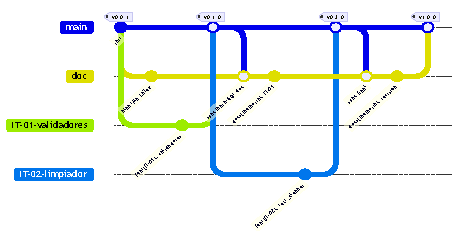
\includegraphics[width=0.8\textwidth]{imagenes/GitFlow.pdf}
          \caption{Estrategia de ramificación y versionado empleada en el desarrollo. Fuente: Elaboración propia.}
          \label{fig:git_flow}
        \end{figure}
        
\end{itemize}


Para garantizar la trazabilidad de las decisiones de diseño a lo largo del tiempo, se ha adoptado el estándar \textit{Conventional Commits} \cite{conventionalcommits}. Esta convención impone una estructura estandarizada para cada entrega de código, facilitando la lectura semántica del historial del proyecto. El formato base utilizado es \texttt{tipo(ámbito): descripción}, donde el ámbito corresponde al identificador de la historia técnica en curso (ej. \texttt{IT-05}).

Para clasificar semánticamente los cambios, los tipos de confirmación (\textit{commits}) se han restringido a la siguiente taxonomía:
\begin{itemize}                                                                                                                                                                  
  \item \textbf{\texttt{feat}:} Incorporación de una nueva funcionalidad al sistema (ej. implementación de un nuevo módulo de extracción o lógica de procesamiento).
  \item \textbf{\texttt{fix}:} Corrección de errores o fallos detectados en el código existente.
  \item \textbf{\texttt{docs}:} Creación o actualización de documentación, incluyendo la redacción de la presente memoria y el registro de decisiones arquitectónicas (ADR).
  \item \textbf{\texttt{test}:} Adición o corrección de pruebas automatizadas, asegurando la no regresión sin alterar el código de producción.
  \item \textbf{\texttt{refactor}:} Reestructuración interna del código que mejora su legibilidad, diseño o rendimiento, sin añadir nuevas funcionalidades ni corregir errores externos.
  \item \textbf{\texttt{chore}:} Tareas de mantenimiento, actualización de dependencias o configuración de las herramientas de integración continua.
\end{itemize}

Cada entrega de código exige no solo el título estandarizado que describe \textit{qué} se ha modificado, sino un cuerpo explicativo obligatorio que documenta con claridad \textit{por qué} se ha tomado dicha decisión técnica frente a otras alternativas.

Asimismo, para proteger la integridad de esta trazabilidad, las fusiones a la rama principal (\texttt{main}) se realizan exclusivamente mediante confirmaciones de fusión explícitas (\textit{Merge Commits}). Se ha descartado la técnica de aplastamiento (\textit{Squash}) al fusionar las ramas efímeras, garantizando que la historia atómica y el razonamiento de cada paso del desarrollo se conserven de manera inmutable.

\subsection{Integración Continua (CI) y automatización de pruebas}
El aseguramiento del correcto funcionamiento del \textit{software} se apoya en un sistema de Integración Continua (CI) desplegado a través de \textit{GitHub Actions}. Este sistema intercepta cada actualización del repositorio y ejecuta automáticamente una batería de pruebas unitarias implementadas con \texttt{pytest}\cite{pytest}.

Un principio de esta metodología ha sido la validación contra la realidad. Las pruebas de los módulos de extracción web (\glr{spiders}{spider}) no se basan en datos inventados o simulados, sino en conjuntos de datos de prueba predefinido, estático y reales en HTML descargados de la web de la Escuela Politécnica Superior de Jaén. Esto garantiza que las pruebas verifiquen el comportamiento del código ante las verdaderas anomalías de la fuente.

Cabe destacar que, debido al alcance académico del proyecto y a la ausencia de un entorno de producción al público (una página web subida a un \textit{hosting}), el enfoque de este trabajo se limita estrictamente a la Integración Continua (CI), excluyendo las prácticas de Despliegue Continuo (CD), lo que permite concentrar los recursos en la experimentación y métricas de evaluación del modelo de lenguaje.

\subsection{Criterios de finalización (Definición de Hecho)}
\label{secc:dod}
Para evitar la ambigüedad sobre el estado de avance del TFG, se ha establecido una estricta \textbf{Definición de Hecho} (\textit{Definition of Done}). Una tarea (cada una de las tarjetas con identificador empezando por IT-XX) solo se considera finalizada y se fusiona en el sistema si cumple simultáneamente seis condiciones:
\begin{enumerate}                                                                                                                                                                  
  \item \textbf{Funcionalidad:} El código cumple el objetivo técnico estipulado.
  \item \textbf{Pruebas:} Incluye casos de prueba exitosos basados en datos reales de la fuente.
  \item \textbf{Documentación:} El código incorpora cadenas de documentación (\textit{docstrings}) formateadas según el estándar \textit{Google Style}\cite{googlestyle} y las convenciones oficiales de Python (PEP 257)\cite{pep257}.
  \item \textbf{Integración:} La funcionalidad pasa las pruebas automáticas en la nube (CI en verde).
  \item \textbf{Defendibilidad:} La decisión técnica subyacente es justificable y defendible con evidencia.
  \item \textbf{Memoria:} La justificación técnica, las métricas o los descubrimientos derivados de la tarea han sido volcados en el borrador de la memoria académica.
\end{enumerate}


\section{Planificación temporal}

Dado el enfoque ágil y experimental de este Trabajo Fin de Grado, la planificación temporal huye de las estimaciones predictivas rígidas tradicionales (como el modelo en cascada). Un sistema RAG requiere iteración y ajuste continuo ante los datos descubiertos, por lo que una planificación lineal resultaría irreal. En su lugar, se ha optado por una estrategia de planificación a dos niveles: una macro-planificación orientada a hitos de entrega y una micro-planificación diaria basada en flujo continuo.

\subsection{Micro-planificación: Tablero Kanban}

La ejecución del día a día se rige por un tablero \textbf{Kanban} implementado mediante \textit{GitHub Projects}. Este tablero refleja el estado en tiempo real de las 61 historias técnicas de usuario (IT-01 a IT-61) que componen el \textit{backlog} del proyecto.

Como se observa en la Figura \ref{fig:tablero_kanban}, el flujo de trabajo se divide en columnas que representan el ciclo de vida de cada tarea. La regla principal de esta micro-planificación es el límite de Trabajo en Curso (\glr{Work In Progress}{WIP}, WIP), que impide iniciar nuevas tareas sin haber cerrado las anteriores. Esto garantiza un avance constante, previniendo el estancamiento y asegurando el cumplimiento estricto de la Definición de Hecho expuesta en la sección anterior.

\begin{figure}[htbp]
  \centering
  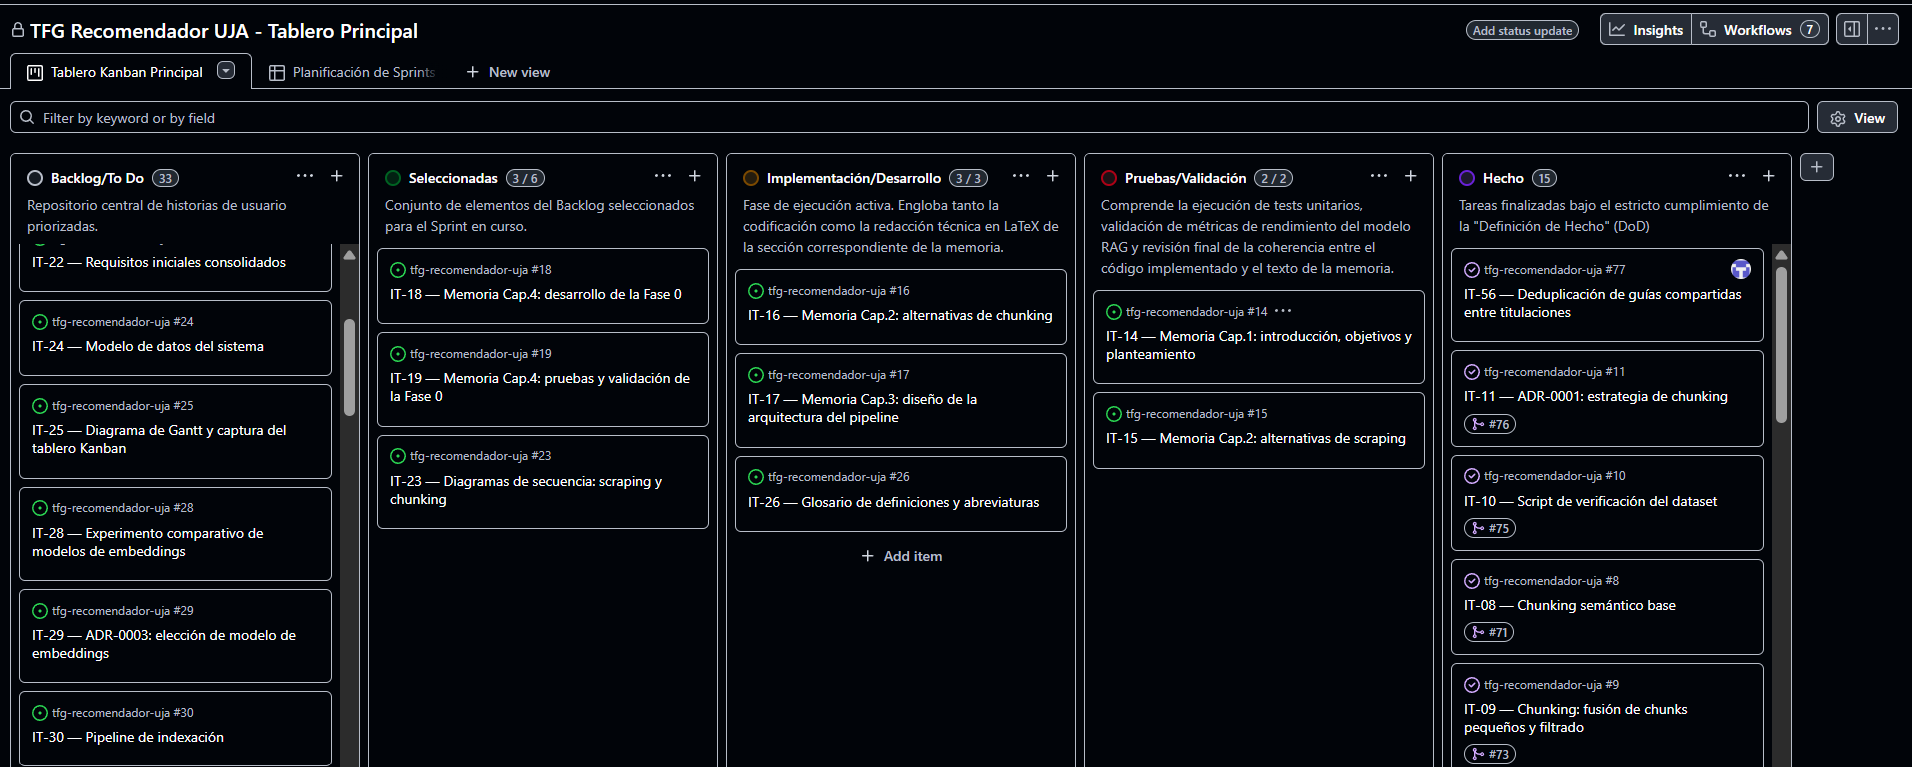
\includegraphics[width=1 \textwidth]{imagenes/tableroKanBan.png}
  \caption{Captura del tablero Kanban utilizado para la gestión ágil del proyecto en GitHub Projects. Fuente: Elaboración propia.}
  \label{fig:tablero_kanban}
\end{figure}

\subsection{Macro-planificación: Hitos y fases (Gantt)}

Para proporcionar una visión global del cronograma y asegurar la viabilidad del proyecto de cara a la fecha de entrega del proyecto, el \textit{backlog} se ha agrupado en seis fases lógicas de desarrollo.

Esta macro-planificación iterativa se ilustra en el diagrama de Gantt de la Figura \ref{fig:gantt}, estructurado de la siguiente manera:
\begin{itemize}                                                                                                                                                                  
  \item \textbf{Fase 0 (Minería de datos y extracción):} Abarca el desarrollo de los rastreadores web (\textit{spiders} en Scrapy), los validadores lógicos, los módulos de limpieza de texto y la fragmentación semántica preliminar (\textit{chunking}).
  \item \textbf{Fase 1 (Incrustaciones y base vectorial):} Comprende la experimentación para la selección del modelo de \textit{embeddings} y el despliegue de la base de datos vectorial local.
  \item \textbf{Fase 2 (Pipeline RAG y LLM):} Consiste en el diseño del \textit{prompt} del sistema, la selección e integración del modelo de lenguaje grande y la evaluación cuantitativa exhaustiva de las respuestas generadas.
  \item \textbf{Fase 3 (Aplicación web de chat):} Diseño de la arquitectura e implementación de la interfaz conversacional accesible (sin registro) y su conexión con el \textit{backend}.
  \item \textbf{Fase 4 (Validación experimental):} Pruebas del sistema con usuarios reales (estudiantes de perfil preuniversitario) y estudios de ablación sobre los hiperparámetros del sistema.
  \item \textbf{Fase 5 (Cierre y memoria):} Volcado final de documentación técnica, revisión de los resultados experimentales y preparación del material de defensa oral (Aunque la memoria se está haciendo a la par que el desarrollo).
\end{itemize}




% Confirmado el 16/07/2026 contra el calendario oficial real de la EPSJ:
% Extraordinaria II del curso 2025/26 (entrega 3/9/2026, defensa 9/9/2026).
% Día 1 del diagrama = 24/06/2026; día 72 = 3/9/2026 (entrega).
\begin{figure}[htbp]
  \centering
  \resizebox{\textwidth}{!}{%
    \begin{ganttchart}[                                                                                                                                                                  
        hgrid, vgrid,
        bar/.append style={fill=blue!40},
        bar height=0.5,
        title height=1,
        y unit chart=0.7cm,
        x unit=0.115cm
      ]{1}{72}
      \gantttitle{Junio}{7}
      \gantttitle{Julio}{31}
      \gantttitle{Agosto}{31}
      \gantttitle{Sept.}{3} \\
      \ganttbar{F0 · Cimientos}{1}{17} \\
      \ganttbar{F1 · Embeddings y vector DB}{18}{31} \\
      \ganttbar{F2 · Pipeline RAG}{32}{48} \\
      \ganttbar{F3 · Aplicación web}{49}{59} \\
      \ganttbar{F4 · Validación y ablation}{60}{68} \\
      \ganttbar{F5 · Cierre y defensa}{69}{72} \\
      \ganttmilestone{Entrega}{72}
    \end{ganttchart}%
  }
  \caption{Planificación temporal del proyecto por fases, ajustada a la
    Extraordinaria II del curso 2025/26 (entrega el 3 de septiembre de 2026).
    Fuente: Elaboración propia.}
  \label{fig:gantt}
\end{figure}







\section{Priorización y estimación del esfuerzo}

El \textit{backlog} del proyecto está formado por 61 historias de usuario
(IT-01 a IT-61). Para decidir en qué orden abordarlas se han combinado dos
criterios independientes: cuánto valor aporta cada una al resultado final y
cuánto esfuerzo cuesta.

\subsection{Priorización por valor: MoSCoW}

El valor se ha clasificado con la técnica \textbf{MoSCoW}~\cite{moscow}, que
divide las tareas en cuatro categorías según su necesidad real para el
proyecto:

\begin{itemize}                                                                                                                                                                  
  \item \textbf{\textit{Must have} (imprescindible):} sin esta tarea el
        sistema no funciona o la memoria no es defendible. Aquí están el rastreo de la
        web, la fragmentación de los textos, la elección experimental de los
        modelos y la evaluación cuantitativa del sistema.
  \item \textbf{\textit{Should have} (importante):} aporta valor claro y se
        hará salvo que el tiempo lo impida, pero su ausencia no invalida el
        resultado.
  \item \textbf{\textit{Could have} (deseable):} mejora el trabajo si sobra
        tiempo.
  \item \textbf{\textit{Won't have} (descartado):} queda explícitamente fuera
        del alcance, como el despliegue en producción o la extensión al resto de
        facultades de la Universidad de Jaén.
\end{itemize}

Esta clasificación tiene una consecuencia práctica: ante un retraso, se sacrifica
primero lo \textit{could} y después lo \textit{should}, pero nunca lo
\textit{must}. El reparto actual es de 37 historias \textit{must},
20 \textit{should} y 4 \textit{could}. Este reparto no es una foto fija:
el \textit{backlog} es un artefacto vivo y ha crecido durante el desarrollo
(las historias IT-57 a IT-61 se añadieron al descubrir necesidades nuevas o
al dividir historias que mezclaban trabajos de naturaleza distinta).

\begin{borrador}                                
  \item \textbf{Fase:} 5 (IT-52) --- cifras a refrescar al cerrar la memoria.
  El \textit{backlog} crece continuamente y las cifras del texto se han
  quedado atrás.
\end{borrador}

\subsection{Estimación del esfuerzo: tallas de camiseta}

Para estimar el coste se ha empleado la técnica de las \textbf{tallas de
  camiseta} (\textit{t-shirt sizing}), que asigna a cada historia una talla
relativa en lugar de una cifra de horas. Se ha elegido esta técnica
deliberadamente: las estimaciones en horas dan una falsa sensación de precisión y,
en un trabajo con una fuerte componente de investigación (donde una tarde puede
irse en descubrir que la web codifica mal sus propias páginas), resultan poco
fiables. Comparar tamaños relativos es más honesto y, sobre todo, más útil.

Las tallas empleadas son:

\begin{itemize}                                                                                                                                                                  
  \item \textbf{XS:} tarea mecánica, sin decisiones de diseño (por ejemplo,
        generar un diagrama a partir del código).
  \item \textbf{S:} una sola unidad de trabajo bien acotada, resoluble en una
        sesión (un script pequeño con sus pruebas, o un registro de decisión).
  \item \textbf{M:} exige varias sesiones o tomar decisiones de diseño no
        triviales (una araña que debe lidiar con anomalías de la fuente).
  \item \textbf{L:} implica experimentación con resultados abiertos: no se
        sabe de antemano cuánto costará porque depende de lo que muestren los datos
        (la comparativa de modelos de incrustaciones o la evaluación del sistema
        completo).
\end{itemize}

El cruce de ambos criterios es lo que gobierna el orden de trabajo: una historia
\textit{must} de talla L (como la evaluación cuantitativa) se planifica con
antelación y se le reserva más tiempo, mientras que una \textit{could} de talla L
sería la primera candidata a quedar fuera.

\subsection{Relación de historias de usuario}

La Tabla~\ref{tab:backlog} recoge el \textit{backlog} completo agrupado por
fases. Cada historia se identifica con un código IT-XX que se usa en todo el proyecto: da nombre a la rama de trabajo, aparece en el
ámbito de cada confirmación de código (\texttt{feat(IT-05): \ldots}) y etiqueta
la incidencia correspondiente en el repositorio, de modo que cualquier línea de
código puede rastrearse hasta la necesidad que la originó.


\small
\begin{xltabular}{\textwidth}{@{}l Y l c c@{}}
  \caption{Relación de historias de usuario del proyecto, agrupadas por fase.}
  \label{tab:backlog} \\
  \toprule
  \textbf{ID} & \textbf{Historia} & \textbf{Tipo} & \textbf{Esfuerzo} & \textbf{Prioridad} \\
  \midrule
  \endfirsthead
  \multicolumn{5}{@{}l}{\small\textit{(continuación de la página anterior)}} \\
  \toprule
  \textbf{ID} & \textbf{Historia} & \textbf{Tipo} & \textbf{Esfuerzo} & \textbf{Prioridad} \\
  \midrule
  \endhead
  \hline
  \multicolumn{5}{r@{}}{\small\textit{(continúa en la página siguiente)}} \\
  \endfoot
  \bottomrule
  \endlastfoot
  \multicolumn{5}{@{}l}{\textbf{Fase 0 — Cimientos: datos, scraping y fragmentación}} \\[2pt]
  IT-01 & Modelos de datos y validadores & Código & S & MUST \\
  IT-02 & Limpiador de texto (TextCleaner) & Código & S & MUST \\
  IT-03 & Spider: listado de grados de la EPSJ & Código & S & MUST \\
  IT-04 & Spider: portada de grado y detección de doble grado & Código & S & MUST \\
  IT-05 & Spider: tabla híbrida de asignaturas & Código & M & MUST \\
  IT-06 & Spider: extracción de guía docente & Código & M & MUST \\
  IT-07 & Spider: salidas profesionales & Código & S & MUST \\
  IT-08 & Chunking semántico base & Código & M & MUST \\
  IT-09 & Chunking: fusión de chunks pequeños y filtrado & Código & S & MUST \\
  IT-10 & Script de verificación del dataset & Código & S & MUST \\
  IT-11 & ADR-0001: estrategia de chunking & ADR & S & MUST \\
  IT-12 & ADR-0002: elección de Scrapy frente a alternativas & ADR & S & MUST \\
  IT-13 & README + empaquetado del proyecto & Gestión & XS & MUST \\
  IT-14 & Memoria Cap.1 y Cap.3: introducción, objetivos y planteamiento & Memoria & M & MUST \\
  IT-15 & Memoria Cap.4: alternativas de scraping & Memoria & S & SHOULD \\
  IT-16 & Memoria Cap.4: alternativas de chunking & Memoria & S & SHOULD \\
  IT-17 & Memoria Cap.4: diseño de la arquitectura del pipeline & Memoria & M & MUST \\
  IT-63 & Memoria Cap.4: implementación del spider de extracción & Memoria & M & MUST \\
  IT-64 & Memoria Cap.4: implementación del chunker y deduplicación & Memoria & S & MUST \\
  IT-19 & Memoria Cap.4: verificación y reproducibilidad de la Fase 0 & Memoria & S & MUST \\
  IT-20 & Estudio de alternativas y viabilidad & Memoria & M & SHOULD \\
  IT-21 & Hipótesis y restricciones & Memoria & XS & SHOULD \\
  IT-22 & Requisitos de usuario & Memoria & S & SHOULD \\
  IT-23 & Diagramas de secuencia: scraping y chunking & Memoria & M & SHOULD \\
  IT-24 & Modelo de datos del sistema & Memoria & S & SHOULD \\
  IT-25 & Diagrama de Gantt y captura del tablero Kanban & Memoria & XS & SHOULD \\
  IT-26 & Glosario de definiciones y abreviaturas & Memoria & S & SHOULD \\
  IT-55 & Pipeline CI/CD: validación semanal del dataset & Gestión & S & MUST \\
  IT-56 & Deduplicación de guías compartidas entre titulaciones & Código & M & MUST \\
  IT-57 & Sincronizar estructura de memoria desde Overleaf & Gestión & XS & SHOULD \\
  IT-60 & Quitar del CI la verificación de un dataset no versionado & Gestión & XS & MUST \\
  IT-61 & Correcciones de la primera revisión del tutor sobre la memoria & Memoria & M & MUST \\
  IT-62 & Segunda ronda de revisión de la memoria & Memoria & M & SHOULD \\
  IT-65 & DQA-0001: anomalías de la fuente de datos EPSJ & DQA & S & MUST \\
  \addlinespace
  \multicolumn{5}{@{}l}{\textbf{Fase 1 — Incrustaciones y base de datos vectorial}} \\[2pt]
  IT-27 & Diseño del conjunto de evaluación (preguntas etiquetadas) & Experimento & M & MUST \\
  IT-28 & Experimento comparativo de modelos de embeddings & Experimento & L & MUST \\
  IT-29 & ADR-0003: elección de modelo de embeddings & ADR & S & MUST \\
  IT-30 & Pipeline de indexación & Código & M & MUST \\
  IT-31 & Experimento comparativo de vector DB & Experimento & M & MUST \\
  IT-32 & ADR-0004: elección de vector DB & ADR & S & MUST \\
  IT-33 & Memoria Cap.4: desarrollo de la Fase 1 & Memoria & M & MUST \\
  IT-59 & Requisitos de sistema (especificación técnica) & Memoria & S & SHOULD \\
  IT-66 & Revisión macro/micro de la memoria al cerrar la Fase 0 & Memoria & S & SHOULD \\
  IT-67 & Spider: detectar respuestas que no son HTML (guías en PDF) & Código & M & MUST \\
  IT-68 & Memoria Cap.4: canalización de indexación & Memoria & S & MUST \\
  IT-69 & Memoria Cap.5: diseño del conjunto de evaluación & Memoria & S & MUST \\
  \addlinespace
  \multicolumn{5}{@{}l}{\textbf{Fase 2 — Pipeline RAG y evaluación}} \\[2pt]
  IT-34 & Diseño del prompt de generación & Código & S & MUST \\
  IT-35 & Elección y configuración del LLM de generación & Experimento & M & MUST \\
  IT-36 & ADR-0005: elección del LLM de generación & ADR & S & MUST \\
  IT-37 & Implementación del pipeline RAG completo & Código & L & MUST \\
  IT-38 & Evaluación cuantitativa del sistema RAG & Experimento & L & MUST \\
  IT-39 & Amenazas a la validez del experimento de evaluación & Experimento & S & MUST \\
  IT-40 & Memoria Cap.4/5: desarrollo de la Fase 2 y evaluación experimental & Memoria & L & MUST \\
  IT-41 & Diagrama de secuencia del flujo RAG completo & Memoria & S & SHOULD \\
  IT-58 & Memoria Cap.5: caracterización del corpus de la Fase 0 y amenazas a su validez & Memoria & S & MUST \\
  \addlinespace
  \multicolumn{5}{@{}l}{\textbf{Fase 3 — Aplicación web de chat}} \\[2pt]
  IT-42 & Diseño de la arquitectura de la app web & Código & S & SHOULD \\
  IT-43 & Storyboards de la interfaz de chat & Memoria & S & SHOULD \\
  IT-44 & Backend: endpoint de chat conectado al RAG & Código & M & SHOULD \\
  IT-45 & Frontend de chat & Código & M & SHOULD \\
  IT-46 & Memoria Cap.4: desarrollo de la Fase 3 (app web) & Memoria & S & SHOULD \\
  IT-47 & Anexo: documentación técnica de la API & Memoria & S & COULD \\
  \addlinespace
  \multicolumn{5}{@{}l}{\textbf{Fase 4 — Validación y estudio de ablación}} \\[2pt]
  IT-48 & Validación con usuarios reales & Experimento & M & COULD \\
  IT-49 & Estudio de ablation & Experimento & M & SHOULD \\
  IT-50 & Memoria: retroalimentación de usuarios y conclusiones & Memoria & M & SHOULD \\
  IT-51 & Anexo: resultados completos de la validación con usuarios & Memoria & S & COULD \\
  \addlinespace
  \multicolumn{5}{@{}l}{\textbf{Fase 5 — Cierre y defensa}} \\[2pt]
  IT-52 & Revisión formal completa de la memoria & Memoria & M & MUST \\
  IT-53 & Material de apoyo para la defensa + ensayo oral & Gestión & S & SHOULD \\
  IT-54 & Anexo: instalación y configuración del sistema & Memoria & S & COULD \\
\end{xltabular}
\normalsize




\section{Tecnologías y herramientas}

\begin{borrador}
  \item \textbf{Fase:} 0 en parte, cerrable ya. Falta el párrafo que abre la
        sección: ahora mismo se salta del título 4.4 al 4.4.1 sin decir nada, que
        es justo lo que el tutor marcó en 4.4.2. Bastan cuatro o cinco líneas
        diciendo qué se va a comparar y en qué orden (extracción, PLN y
        alucinaciones, RAG, tipo de modelo, base vectorial) y por qué ese orden
        sigue el recorrido del dato.
  \item Aquí también encaja la tabla herramienta--papel que ya está apuntada en
        un comentario del código fuente, si al final se hace.
\end{borrador}

\subsection{Extracción de datos}
\label{sec:eleccion_herramientas}

\textcolor{borrador2}{El rastreo web (\textit{web scraping}) es el proceso automatizado de descargar páginas y extraer de ellas datos estructurados a partir de su HTML. A alto nivel, una herramienta de rastreo emite una petición HTTP, recibe la respuesta HTML, la analiza (\textit{parsing}) y localiza los datos mediante selectores (CSS o XPath) para, por último, normalizar el resultado. Este proceso rara vez es limpio y uniforme: la codificación de caracteres suele ser inconsistente, la estructura del HTML no es igual entre páginas y, en algunos sitios, el contenido se genera dinámicamente mediante JavaScript. Las tres familias de herramientas que se comparan a continuación resuelven estos problemas con distinto alcance.}

Como lenguaje base se ha utilizado Python en su versión 3.13 y, para la extracción de datos, se han estudiado tres claras opciones, las cuales se comentan en los apartados siguientes.

\subsubsection{Scrapy\cite{scrapy}}

Scrapy\footnote{\url{https://scrapy.org/}} es un \textit{framework} asíncrono completo de \textit{crawling} (rastreo web). Dadas sus características, las cuales se detallan a continuación, ha sido la opción elegida.

\begin{itemize}                                                                                                                                                                  
  \item \textbf{Codificación de textos:} Los objetos \texttt{TextResponse} y \texttt{HtmlResponse} resuelven la codificación automáticamente siguiendo este orden de prioridad:
        \begin{enumerate}                                                                                                                                                                  
          \item Codificación indicada explícitamente al construir la respuesta.
          \item BOM (\textit{Byte Order Mark}) al principio del cuerpo.
          \item Cabecera HTTP \texttt{Content-Type}.
          \item Declaración de codificación dentro del propio documento (etiqueta \texttt{<meta>}).
          \item Autodetección por parte del \textit{framework}.
        \end{enumerate}
        Las guías docentes de la UJA no llevan BOM, por lo que decide la cabecera HTTP: al anteponerla a la etiqueta \texttt{<meta>} del cuerpo, Scrapy decodifica correctamente unas guías servidas en ISO-8859-1 pese a que se declaren como UTF-8, resolviendo el problema de codificación sin necesidad de código adicional.
        
  \item \textbf{Respeto a robots.txt:} Soporte nativo mediante \texttt{ROBOTSTXT\_OBEY = True}, que permite cumplir automáticamente con las directrices de rastreo del sitio.
        
  \item \textbf{Control de tasa (\textit{throttling}):} El \textit{framework} ofrece parámetros de configuración que permiten ajustar el proceso de rastreo para no saturar el servidor objetivo.
        
  \item \textbf{Pruebas sin conexión:} Permite simular respuestas HTML (con cuerpo, URL y cabeceras HTTP) directamente en memoria. Esto facilita la creación de pruebas unitarias sin necesidad de realizar peticiones de red reales.
        
  \item \textbf{Madurez y soporte:} Es un \textit{framework} de referencia en la industria, mantenido activamente. Además, desde la serie 2.13, incluye soporte de tipado estático nativo (\texttt{py.typed}) conforme al estándar PEP 561.\cite{scrapydocs}
        
  \item \textbf{Desventaja:} Presenta una curva de aprendizaje inicial más pronunciada debido a su complejidad y al gran número de componentes integrados.
\end{itemize}


\subsubsection{BeautifulSoup\cite{beautifulsoup}}

Combina un \textit{parser} de HTML (BeautifulSoup) con un cliente HTTP (\texttt{requests}).

\begin{itemize}                                                                                                                                                                  
  \item \textbf{Pros:} Gran simplicidad, ideal para tareas pequeñas y estáticas.
  \item \textbf{Contras:} BeautifulSoup no es un rastreador web (no gestiona colas, reintentos ni \textit{rate limiting}); \texttt{requests} no respeta \texttt{robots.txt} automáticamente; el manejo de la codificación (\textit{encoding}) queda completamente en manos del desarrollador. Se considera una herramienta demasiado simple para los requisitos del proyecto.
\end{itemize}

\subsubsection{Selenium \cite{selenium} / Playwright}
Se basa en la automatización de navegadores con renderizado real.

\begin{itemize}                                                                                                                                                                  
  \item \textbf{Pros:} Imprescindibles para Single Page Applications (SPAs) y contenido cargado dinámicamente mediante JavaScript.
  \item \textbf{Contras:} La web de la EPSJ está desarrollada en Drupal con contenido estático. Por tanto, el renderizado de JavaScript es innecesario, lo que haría que el programa fuera más lento y consumiera más recursos de los necesarios.
\end{itemize}

%[jccuevas] \paragraph{Decisión final}
Conforme a lo comentado anteriormente, se adopta \textbf{Scrapy} como herramienta de extracción de datos de webs. La evidencia sobre la gestión correcta de la codificación fue el factor decisivo, reforzado por el soporte nativo de \texttt{robots.txt}, el control de tasa configurable, la testabilidad sin conexión con \texttt{HtmlResponse} y la gran comunidad de soporte. Las alternativas analizadas requerían reimplementar manualmente dichas garantías o estaban sobredimensionadas para un sitio estático.



% Python 3.13, Scrapy (justificado en el ADR-0002), pytest con casos de prueba
% reales, mypy, GitHub Actions. Conviene una tabla: herramienta - papel.

\subsection{Modelos de lenguaje y alucinaciones}

\textcolor{red}{[jccuevas] Lo que te he comentado antes, no pases de un título a otro sin explicar.}

\textcolor{red}{[jccuevas] Lo que vas a detallar aquí está bien, pero dale más profundidad a lo que no veáis en asignaturas, aunque, como mucho, esta parte que te lleve un par de páginas por cada apartado 2.2, 2.3, etc., alguno puede tener más, pero esto no es tu trabajo, es la tecnología, sintetiza.}

El Procesamiento del Lenguaje Natural (PLN, o NLP por sus siglas en inglés) tiene como objetivo dotar a los sistemas informáticos de la capacidad de comprender, interpretar y generar el lenguaje humano de una manera computacionalmente útil\cite{jurafsky2026slp3}. Los transformadores, propuestos por Vaswani et al.\cite{vaswani2017attention}, son la arquitectura estándar hoy en día para construir modelos de lenguaje grandes (LLM): un LLM, en su definición técnica, es un sistema computacional diseñado para predecir la probabilidad de la siguiente palabra a partir de un contexto o historial de palabras anteriores.

Las alucinaciones en la generación de lenguaje natural (NLG, por sus siglas en inglés) son aquellos contenidos generados que carecen de sentido o que no son fieles al texto de origen proporcionado; estas se pueden dividir en dos grandes categorías\cite{ji2023hallucination}:

\begin{itemize}                                                                                                                                                                  
  \item \textbf{Alucinaciones intrínsecas:} El modelo genera información que contradice directamente los datos o el texto proporcionado como fuente.
  \item \textbf{Alucinaciones extrínsecas:} El modelo genera información adicional que no aparece en la fuente original. Aunque esta información inventada pueda ser correcta en el mundo real, se considera alucinación porque no puede ser verificada utilizando únicamente la entrada proporcionada.
\end{itemize}

Uno de los factores por los que los modelos podrían alucinar son los datos de entrada, dado que muchos conjuntos de datos se construyen de forma automatizada, emparejando fuentes con textos de referencia que contienen información extra (por ejemplo, emparejar una tabla de datos de Wikipedia con el primer párrafo del artículo, el cual suele contener más datos que la tabla)\cite{ji2023hallucination}.

Esto podría conllevar una inaceptable mala orientación a futuros estudiantes universitarios: inventar asignaturas, notas de corte o planes de estudio inexistentes. En la Figura~\ref{fig:alucinacion_deepseek} se muestra un \textit{prompt} real enviado a DeepSeek\footnote{\url{https://chat.deepseek.com/}}, un modelo de lenguaje que ha ido ganando popularidad por publicar versiones de pesos abiertos y por los límites amplios de su capa gratuita. Al pedirle todos los grados universitarios que se ofertan actualmente en la Escuela Politécnica Superior de Jaén (EPSJ), la respuesta incluye información falsa: oferta titulaciones que no se imparten en el centro, como el Grado en Ingeniería Civil o el Grado en Ingeniería de Tecnologías Mineras, y las presenta con total seguridad, sin advertir de que puedan ser incorrectas.

\begin{figure}[H]
  \centering
  
\includegraphics[width=0.92\textwidth]{imagenes/Alucinacion1_Deepseek.png}\\[4pt]
  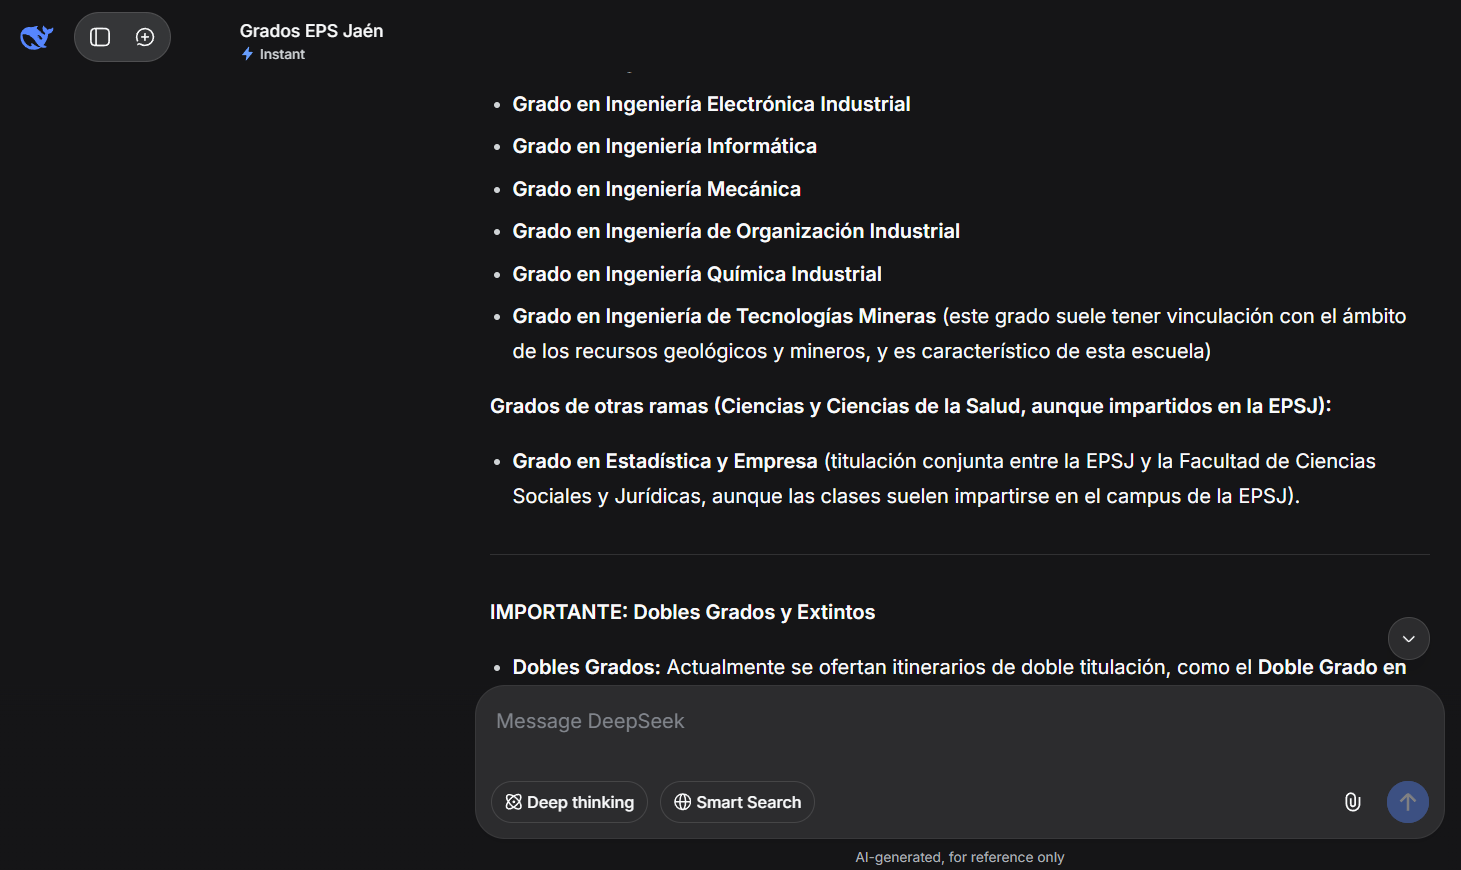
\includegraphics[width=0.92\textwidth]{imagenes/Alucinacion2_Deepseek.png}
  \caption[Ejemplo real de alucinación de un LLM sin RAG]{Respuesta de
    DeepSeek al pedirle la oferta actual de grados de la EPSJ (julio de 2026):
    entre titulaciones reales, el modelo intercala grados que no se imparten
    en el centro, como Ingeniería Civil o Ingeniería de Tecnologías Mineras.
    Fuente: captura propia de la interfaz web de DeepSeek.}
  \label{fig:alucinacion_deepseek}
\end{figure}

Mitigar este riesgo sin renunciar a la naturalidad de la conversación es precisamente lo que persigue la arquitectura de recuperación aumentada por generación (RAG) que se describe en el apartado siguiente: no elimina por completo las alucinaciones, pero las reduce al obligar al modelo a apoyarse en documentos reales.

\subsection{Recuperación aumentada por generación (RAG)}

Los modelos de lenguaje almacenan en sus parámetros parte del conocimiento adquirido durante el entrenamiento. Una vez finalizado este proceso, dicho conocimiento permanece condicionado por los datos utilizados y por la fecha en la que fueron recopilados. Por tanto, el modelo no incorpora automáticamente los cambios que se produzcan con posterioridad (si estos cambiaron) y sus respuestas tampoco incluyen necesariamente una indicación verificable del origen y fecha de la información empleada. Estas limitaciones resultan especialmente relevantes en dominios sujetos a actualizaciones periódicas, como la oferta académica de la universidad, en este caso, la UJA.

La recuperación aumentada por generación fue propuesta por Lewis et al.~\cite{lewis2020rag} como una arquitectura que combina la memoria paramétrica de un modelo de lenguaje con una memoria externa formada por una colección de documentos. Ante una consulta, el sistema recupera primero los textos que considera más relevantes y los proporciona al modelo como contexto para generar la respuesta. De esta forma, el conocimiento almacenado en los parámetros no constituye la única fuente disponible durante la generación.

Este enfoque presenta dos ventajas principales. En primer lugar, permite actualizar la información disponible modificando la colección documental, sin necesidad de volver a entrenar el modelo completo. En segundo lugar, posibilita relacionar las respuestas con los documentos recuperados, lo que mejora su trazabilidad y facilita comprobar si están respaldadas por una fuente. Esta capacidad resulta útil para reducir el problema de las alucinaciones descrito más arriba, aunque no lo elimina por completo: el sistema todavía puede recuperar información poco pertinente, interpretar incorrectamente el contexto o generar afirmaciones que no estén contenidas en él.

Una alternativa sería ajustar los parámetros del modelo con información específica del dominio mediante ajuste fino (\textit{fine-tuning}). Este procedimiento puede resultar adecuado para adaptar el comportamiento, el formato de salida o el desempeño del modelo en una tarea concreta, pero no ofrece por sí solo una referencia explícita a la fuente de cada afirmación. Además, cuando los datos cambian con frecuencia, mantener el conocimiento actualizado exigiría preparar nuevos ejemplos y repetir el proceso de ajuste.

En el contexto de este trabajo, la arquitectura RAG permite separar el modelo de lenguaje de la información oficial de la EPSJ. Los planes de estudio, las guías docentes y las salidas profesionales pueden actualizarse en la colección sin modificar los parámetros del modelo, a la vez que los fragmentos recuperados proporcionan una base documental para las respuestas. No obstante, la calidad final dependerá de todo el proceso: la cobertura y limpieza de la colección, la estrategia de fragmentación, la capacidad del recuperador para seleccionar información pertinente y las instrucciones proporcionadas al modelo durante la generación.

\subsection{Modelos propietarios frente a modelos de pesos abiertos}
\label{subsec:propietarios_abiertos}

Los modelos propietarios son aquellos cuyos pesos no se distribuyen públicamente y a los que se accede normalmente mediante una aplicación o una interfaz de programación de aplicaciones (API) gestionada por el proveedor. GPT (OpenAI)~\cite{openai_api2020}, Claude (Anthropic)~\cite{anthropic_claude2026} y Gemini (Google)~\cite{google_gemini2026} son ejemplos destacados de esta categoría. En este modelo de distribución, la empresa desarrolladora conserva el control sobre los pesos, la infraestructura de ejecución y la información técnica que publica acerca de la arquitectura y del proceso de entrenamiento.

En contraposición, los modelos de pesos abiertos permiten descargar los parámetros aprendidos por la red neuronal y, cuando la licencia y los recursos disponibles lo permiten, ejecutarlos en infraestructura propia. Esta disponibilidad no implica por sí sola que el sistema completo sea de código abierto o software libre, pues el código de entrenamiento, los datos utilizados y otros componentes pueden no publicarse~\cite{osi_osaid2024}. Entre las familias que han publicado versiones con pesos abiertos se encuentran Llama (Meta)~\cite{meta_llama31_license2024}, Mistral (Mistral AI)~\cite{mistral_models2026} y Qwen (Alibaba)~\cite{qwen3_2025}.

La disponibilidad de los pesos puede permitir a usuarios e instituciones desplegar el modelo en equipos propios o en instancias privadas de computación. Cuando tanto la inferencia como el resto del flujo se ejecutan localmente y no intervienen API, telemetría ni otros servicios externos, las consultas pueden mantenerse dentro de una infraestructura controlada por la organización.

En este proyecto de recomendación de grados, la capacidad de mantener bajo control la información introducida durante las conversaciones resulta especialmente relevante, ya que parte del público objetivo podría estar formado por menores de edad.

En este trabajo se prioriza un mayor control sobre la infraestructura y el tratamiento local de las consultas, por su adecuación a los requisitos de privacidad y control del sistema; no obstante, la elección del modelo concreto se realizará posteriormente mediante una evaluación técnica y experimental (Fase 2, IT-35/ADR-0005).

\textcolor{borrador2}{La Figura~\ref{fig:privativos_vs_abiertos} resume el contraste entre ambas familias y sitúa en cada bando las que se citan en este apartado.}

% ------------------------------------------------------------------
% Figura "VS": dos bandos (propietarios vs pesos abiertos) con los nombres
% de cada familia como insignias en un color aproximado de su marca. NO son
% los logotipos oficiales (evita problemas de marca registrada y mantiene la
% figura como elaboración propia): solo identifican visualmente cada familia.
% ------------------------------------------------------------------
\definecolor{marcaOpenAI}{HTML}{10A37F}
\definecolor{marcaClaude}{HTML}{CC785C}
\definecolor{marcaGemini}{HTML}{1A73E8}
\definecolor{marcaLlama}{HTML}{0866FF}
\definecolor{marcaMistral}{HTML}{FA520F}
\definecolor{marcaQwen}{HTML}{615CED}
\begin{figure}[H]
  \centering
  \begin{tikzpicture}[                                                                                                                                                                  
      insignia/.style={rounded corners=4pt, text=white, align=center,
          font=\small\bfseries, minimum width=2.7cm,
          minimum height=0.9cm, inner sep=3pt},
      subt/.style={font=\footnotesize\itshape, align=center, text=black},
      bando/.style={rounded corners=6pt, draw=diagGrupoBorde, fill=diagGrupo,
          inner sep=12pt}
    ]
    % --- Bando izquierdo: modelos propietarios ---
    \node[insignia, fill=marcaOpenAI] (gpt)    at (0,3.1) {GPT\\[-1pt]{\footnotesize\mdseries OpenAI}};
    \node[insignia, fill=marcaClaude] (claude) at (0,1.8) {Claude\\[-1pt]{\footnotesize\mdseries Anthropic}};
    \node[insignia, fill=marcaGemini] (gemini) at (0,0.5) {Gemini\\[-1pt]{\footnotesize\mdseries Google}};
    \node[subt] (subP) at (0,-0.9) {Pesos cerrados\\Acceso mediante API};
    % --- Bando derecho: modelos de pesos abiertos ---
    \node[insignia, fill=marcaLlama]   (llama)   at (7,3.1) {Llama\\[-1pt]{\footnotesize\mdseries Meta}};
    \node[insignia, fill=marcaMistral] (mistral) at (7,1.8) {Mistral\\[-1pt]{\footnotesize\mdseries Mistral AI}};
    \node[insignia, fill=marcaQwen]    (qwen)    at (7,0.5) {Qwen\\[-1pt]{\footnotesize\mdseries Alibaba}};
    \node[subt] (subA) at (7,-0.9) {Parámetros descargables\\Ejecución local · control de los datos};
    % --- VS central ---
    \node[circle, draw=diagNodoBorde, fill=white, line width=1pt,
      minimum size=1.25cm, font=\LARGE\bfseries, text=diagNodoBorde] (vs) at (3.0,1.8) {VS};
    % Paneles de fondo con su título
    \begin{scope}[on background layer]
      \node[bando, fit=(gpt)(gemini)(subP),
        label={[font=\bfseries]north:Modelos propietarios}] {};
      \node[bando, fit=(llama)(qwen)(subA),
        label={[font=\bfseries]north:Modelos de pesos abiertos}] {};
    \end{scope}
  \end{tikzpicture}
  \caption{Modelos de lenguaje propietarios (pesos
    cerrados, acceso mediante la API del proveedor) frente a modelos de pesos
    abiertos (parámetros descargables, ejecución local y control de los datos).
    Los nombres se muestran como insignias identificativas, no como los
    logotipos oficiales de cada marca. Fuente: elaboración propia.}
  \label{fig:privativos_vs_abiertos}
\end{figure}

\subsection{Base de datos vectorial}

\begin{borrador}                                                                                                                                                                  
  \item \textbf{Trasladado desde Antecedentes} (reencuadre del capítulo 2).
  \item \textbf{Fase:} 1 (IT-28/IT-31): panorama de bases de datos vectoriales antes de la comparativa experimental y el ADR-0004.
\end{borrador}

\section{Arquitectura del sistema}

\begin{borrador}                                                                                                                                                                  
  \item \textbf{Faltan:} Concretar los bloques de las Fases 1 a 3 (modelo de incrustaciones, base vectorial, LLM e interfaz) cuando esas decisiones estén tomadas.
\end{borrador}

Como se observa en la Figura~\ref{fig:arquitectura_pipeline}, primero se obtienen los datos necesarios para las recomendaciones (grados, asignaturas, guías y salidas laborales). Antes de fragmentarse, ese texto pasa por el módulo de limpieza, que corrige la codificación y repara las URL rotas de la fuente directamente extraída de la página web oficial. Este paso no aparece como caja propia en la Figura~\ref{fig:arquitectura_pipeline} porque se ejecuta dentro del propio rastreador, sobre cada ítem según se extrae, y no como una etapa posterior independiente. A continuación, el texto se pasa por el fragmentador (\textit{chunker}), que parte este en fragmentos manejables para el modelo de incrustaciones, según se detalla en la Sección~\ref{subsec:chunking}.

\textcolor{red}{No se comienzan los párrafos con 'Y'}

\textcolor{blue}{[sbp] Corregido, y revisado el resto del documento para que no vuelva a ocurrir.}

Con estos trozos de información, se pasa al \textit{embedding} con el que se introducirán los datos en la base de datos vectorial.

%OJO te faltaba una "d" en embedding. 

Por último llega el \textit{pipeline} RAG: tras la pregunta del usuario, el sistema, utilizando como memoria la base de datos vectorial, recupera los fragmentos pertinentes a la pregunta y responde. Con toda esta última fase se podrá interactuar mediante la aplicación web.

Cabe recalcar que el rastreador y el fragmentador son dos módulos independientes: el primero no sabe nada de cómo se va a fragmentar el texto que extrae, y el segundo no sabe nada de cómo se obtuvo el texto que recibe, solo que le llega el fichero que contiene todos los datos en crudo. Esta separación es intencionada: volver a fragmentar es una operación barata que se repite muchas veces durante la experimentación, mientras que volver a rastrear la web es costosa y hace peticiones costosas, por lo que hay que ser respetuoso con el servidor de la universidad, el razonamiento completo, con la evidencia que lo sostiene, se recoge en la Sección~\ref{secc:verificacion_fase0} y en el ADR-0001.

\textcolor{red}{La imagen es poco legible, el texto es muy pequeño}

\textcolor{blue}{[sbp] Corregido: he ampliado la figura del 50\% al 90\% del ancho de página. Si no es lo suficientemente legible igual debería escalar la fuente.}



\begin{figure}[H]
  \centering
  \resizebox{\textwidth}{!}{%
    \begin{tikzpicture}[node distance=0.55cm and 1cm]
      % Fase 0
      \node[nodoDiag] (web) {Web pública\\EPSJ};
      \node[nodoDiag, below=of web] (grados) {\texttt{grados.json}};
      \node[nodoDiag, below=of grados] (chunks) {\texttt{chunks.json}};
      % Fase 1
      \node[nodoDiag, right=3.4cm of web] (emb) {Modelo de\\\textit{embeddings}};
      \node[nodoDiag, cylinder, shape border rotate=90, aspect=0.15, below=of emb] (bd) {Base de datos\\vectorial};
      % Fase 2
      \node[nodoDiag, right=3cm of emb] (preg) {Pregunta\\del usuario};
      \node[nodoDiag, below=of preg] (rec) {Recuperación\\de fragmentos};
      \node[nodoDiag, below=of rec] (llm) {LLM local};
      \node[nodoDiag, below=of llm] (resp) {Respuesta\\fundamentada};
      % Fase 3
      \node[nodoDiag, right=3.2cm of rec] (chat) {Interfaz de chat\\sin registro};
      % Nodos invisibles que "miden" cada título (mismo texto y fuente que la
      % etiqueta real) para que el fit incluya su ancho: un label de TikZ no
      % forma parte del cálculo del área del nodo, así que sin esto el título
      % puede sobresalir de la caja aunque esta se ensanche.
      \node[font=\small, inner sep=0pt, text opacity=0, above=1pt of web] (f0medida) {Fase 0 --- Colección de datos};
      \node[font=\small, inner sep=0pt, text opacity=0, above=1pt of emb] (f1medida) {Fase 1 --- Indexación};
      \node[font=\small, inner sep=0pt, text opacity=0, above=1pt of preg] (f2medida) {Fase 2 --- \textit{Pipeline} RAG};
      \node[font=\small, inner sep=0pt, text opacity=0, above=1pt of chat] (f3medida) {Fase 3 --- Aplicación web};
      % Cajas de fase (en la capa de fondo, para no tapar los nodos)
      \begin{scope}[on background layer]
        \node[grupoDiag, inner xsep=20pt, inner ysep=16pt, fit=(web)(grados)(chunks)(f0medida), label={[tituloGrupo]north:Fase 0 --- Colección de datos}] (f0) {};
        \node[grupoDiag, inner xsep=20pt, inner ysep=16pt, fit=(emb)(bd)(f1medida), label={[tituloGrupo]north:Fase 1 --- Indexación}] (f1) {};
        \node[grupoDiag, inner xsep=20pt, inner ysep=16pt, fit=(preg)(rec)(llm)(resp)(f2medida), label={[tituloGrupo]north:Fase 2 --- \textit{Pipeline} RAG}] (f2) {};
        \node[grupoDiag, inner xsep=20pt, inner ysep=16pt, fit=(chat)(f3medida), label={[tituloGrupo]north:Fase 3 --- Aplicación web}] (f3) {};
      \end{scope}
      % Flechas internas
      \draw[flechaDiag] (web) -- node[right, font=\footnotesize]{\textit{spider} (Scrapy)} (grados);
      \draw[flechaDiag] (grados) -- node[right, font=\footnotesize]{\textit{chunker}} (chunks);
      \draw[flechaDiag] (emb) -- (bd);
      \draw[flechaDiag] (preg) -- (rec);
      \draw[flechaDiag] (rec) -- (llm);
      \draw[flechaDiag] (llm) -- (resp);
      % Flechas entre fases
      \draw[flechaDiag] (chunks.east) -- (emb.west);
      \draw[flechaDiag] (bd.east) -- (rec.west);
      \draw[flechaDiag] (resp.east) -- (chat.south west);
    \end{tikzpicture}%
  }
  \caption{Arquitectura general del sistema, organizada por fases de
    desarrollo. Fuente: Elaboración propia.}
  \label{fig:arquitectura_pipeline}
\end{figure}

\section{Diseño de los datos}


El diagrama de clases de la Figura~\ref{fig:modelo_datos} recoge las diferentes estructuras de datos de la aplicación, que pueden dividirse en dos partes claras: la primera es la de los datos en crudo extraídos de la web, como la relacionada con los grados y las asignaturas, cada cual con su guía docente (si está disponible) y sus salidas. Toda esta información converge y se trocea para dar lugar a los fragmentos (\textit{chunks}), que además contienen un entero que indica en cuántos trozos totales se ha dividido la unidad original (asignatura, salida o guía) y el índice del trozo de información.

\begin{figure}[H]
  \centering
  \resizebox{0.95\textwidth}{!}{%
    \begin{tikzpicture}[                                                                                                                                                                  
        node distance=1.1cm and 1.4cm,
        clase/.style={rectangle split, rectangle split parts=2,
            draw=diagNodoBorde, fill=diagNodo, align=left,
            font=\footnotesize, inner sep=5pt},
        etiqRel/.style={font=\scriptsize, fill=white, inner sep=1.5pt},
        mult/.style={font=\scriptsize, inner sep=1pt}
      ]
      % Entidades
      \node[clase] (grado) {\textbf{Grado}
        \nodepart{two}
        nombre: \texttt{str}\\
        url: \texttt{str}\\
        es\_doble\_grado: \texttt{bool}};
      \node[clase, below left=of grado] (asig) {\textbf{Asignatura}
        \nodepart{two}
        grado: \texttt{str}\\
        codigo: \texttt{str}\\
        nombre: \texttt{str}\\
        tipo\_asignatura: \texttt{str}\\
        ects: \texttt{float}\\
        ofertada: \texttt{bool}\\
        tiene\_guia: \texttt{bool}\\
        menciones: \texttt{list}};
      \node[clase, below right=of grado] (salidas) {\textbf{Salidas}
        \nodepart{two}
        grado: \texttt{str}\\
        texto: \texttt{str}};
      \node[clase, below=of asig] (guia) {\textbf{Guía}
        \nodepart{two}
        grado: \texttt{str}\\
        codigo: \texttt{str}\\
        nombre: \texttt{str}\\
        resumen: \texttt{str}\\
        temario: \texttt{str}\\
        fallback: \texttt{bool}};
      \node[clase, below=3.2cm of salidas] (chunk) {\textbf{Chunk}
        \nodepart{two}
        origen: \texttt{str}\\
        grados: \texttt{list}\\
        codigos: \texttt{list}\\
        nombre: \texttt{str}\\
        texto: \texttt{str}\\
        chunk\_index: \texttt{int}\\
        total\_chunks: \texttt{int}};
      % Relaciones
      \draw[flechaDiag] (grado.south west) -- node[etiqRel]{ofrece}
      node[mult, pos=0.1, left]{1} node[mult, pos=0.92, above right]{*} (asig.north);
      \draw[flechaDiag] (grado.south east) -- node[etiqRel]{tiene}
      node[mult, pos=0.1, right]{1} node[mult, pos=0.9, above left]{0..1} (salidas.north);
      \draw[flechaDiag] (asig.south) -- node[etiqRel]{documentada por}
      node[mult, pos=0.08, right]{1} node[mult, pos=0.92, right]{0..1} (guia.north);
      \draw[flechaDiag] (guia.east) -- node[etiqRel]{troceada y deduplicada en}
      node[mult, pos=0.08, above]{*} node[mult, pos=0.9, above]{*} (chunk.west);
      \draw[flechaDiag] (salidas.south) -- node[etiqRel]{troceada en}
      node[mult, pos=0.08, right]{1} node[mult, pos=0.9, right]{*} (chunk.north);
    \end{tikzpicture}%
  }
  \caption{Modelo de datos conceptual de las entidades extraídas mediante
    \textit{web scraping}. Fuente: Elaboración propia.}
  \label{fig:modelo_datos}
\end{figure}

\section{Fase 0: construcción de la colección documental}

\subsection{Situación de partida}

Para crear la arquitectura RAG propuesta, el requisito indispensable es disponer de la información oficial de manera precisa y actualizada. La EPSJ publica de forma abierta todos estos datos relativos a sus planes de estudio en su portal web oficial\cite{epsj_grados}. No obstante, un análisis técnico a nivel de código (sobre todo HTML) preliminar de estas fuentes revela deficiencias estructurales que imposibilitan la búsqueda automatizada directa por parte de la IA.

Durante el estudio de la fuente de datos, se han documentado los siguientes obstáculos técnicos:

\begin{itemize}                                                                                                                                                                  
  \item \textbf{Inconsistencia en la estructura de navegación:} Las rutas (URLs) de acceso a las distintas titulaciones presentan patrones irregulares y \textit{slugs} inconsistentes en el cuerpo de las páginas.
  \item \textbf{Tablas de datos híbridas y heterogéneas:} La relación de asignaturas no sigue un esquema tabular único. Se combinan listas de materias troncales con tablas de optativas agrupadas por mención, lo que provoca duplicidades en la fuente. Además, no existe una nomenclatura estandarizada entre planes (por ejemplo, el Trabajo Fin de Grado recibe clasificaciones distintas según la antigüedad de la titulación).
  \item \textbf{Ruido tipográfico y errores nativos de enlace:} En el código fuente se ha detectado la presencia de caracteres invisibles (espacios de no separación o de ancho cero) e iconos incrustados en el texto. Asimismo, la plataforma presenta errores de generación nativos, tales como URLs de guías docentes con sufijos duplicados (ej. \texttt{\dots\_es.htmles.html}) que derivan en enlaces rotos.
  \item \textbf{Datos incompletos y registros de relleno:} En titulaciones de reciente implantación (como el Grado en Inteligencia Artificial y Ciberseguridad), materias de cursos superiores carecen aún de guía docente publicada. Paralelamente, en las tablas de matriculación aparecen filas de relleno con nombres genéricos (ej. <<Optativa 1>>), sin código oficial, que no representan asignaturas reales.
\end{itemize}

Cada una de estas anomalías, con la evidencia real que la respalda y el tratamiento aplicado en el código, se documenta en el registro DQA-0001\cite{repo_tfg}, aquí se recogen solo a alto nivel para no desviar la memoria hacia el detalle de problemas puntuales.

\subsection{Justificación del enfoque técnico}

Por todo esto, se decidió desarrollar el primer bloque de este proyecto: la implementación de un motor de extracción personalizado (\textit{web scraper}) y de limpieza de texto.

Alimentar un sistema RAG con datos ruidosos o enlaces rotos desencadenaría el antipatrón \textit{Garbage In, Garbage Out} (basura entra, basura sale). Por tanto, es obligatorio desplegar una fase inicial de recolección de datos que actúe como filtro determinista. Solo mediante la validación de filas, la limpieza de caracteres anómalos y la reparación de enlaces rotos, se puede asegurar que la base de datos vectorial sobre la que operará la Inteligencia Artificial contenga una fuente de conocimiento íntegro y de alta calidad.


\subsection{Extracción del catálogo de titulaciones y asignaturas}


En la Figura~\ref{fig:secuencia_scraping} se detalla la secuencia de peticiones entre el
rastreador (\textit{spider}) y la página web, así como las posibles alteraciones que puede tener este flujo dependiendo de si el objeto actual es un doble grado o uno simple.

El rastreador no hace una única petición, sino que encadena varias, una por cada tipo de página de la web: primero el listado de titulaciones, siguiendo siempre el enlace de cada grado, después la portada de cada grado, donde se identifica si es un doble grado con el nombre, a continuación la tabla de asignaturas, y por cada asignatura con enlace propio, su guía docente. El flujo se bifurca en tres puntos, todos recogidos en la figura: una asignatura puede tener guía docente publicada o no tenerla, una guía puede presentar la estructura esperada o, si no aparece, recurrir a un resumen general de la página en lugar de descartar la asignatura, y un grado puede ser simple, se extraen sus salidas profesionales propias, o doble, cuyas salidas se construyen a posteriori puesto que son exactamente la unión de las de sus dos grados base.

\textcolor{red}{[jccuevas] Igual que antes un poco pequeño el texto. No tengas miedo de usar más espacio para que el texto sea legible.}

\textcolor{blue}{[sbp] Corregido}


\begin{figure}[H]
  \centering
  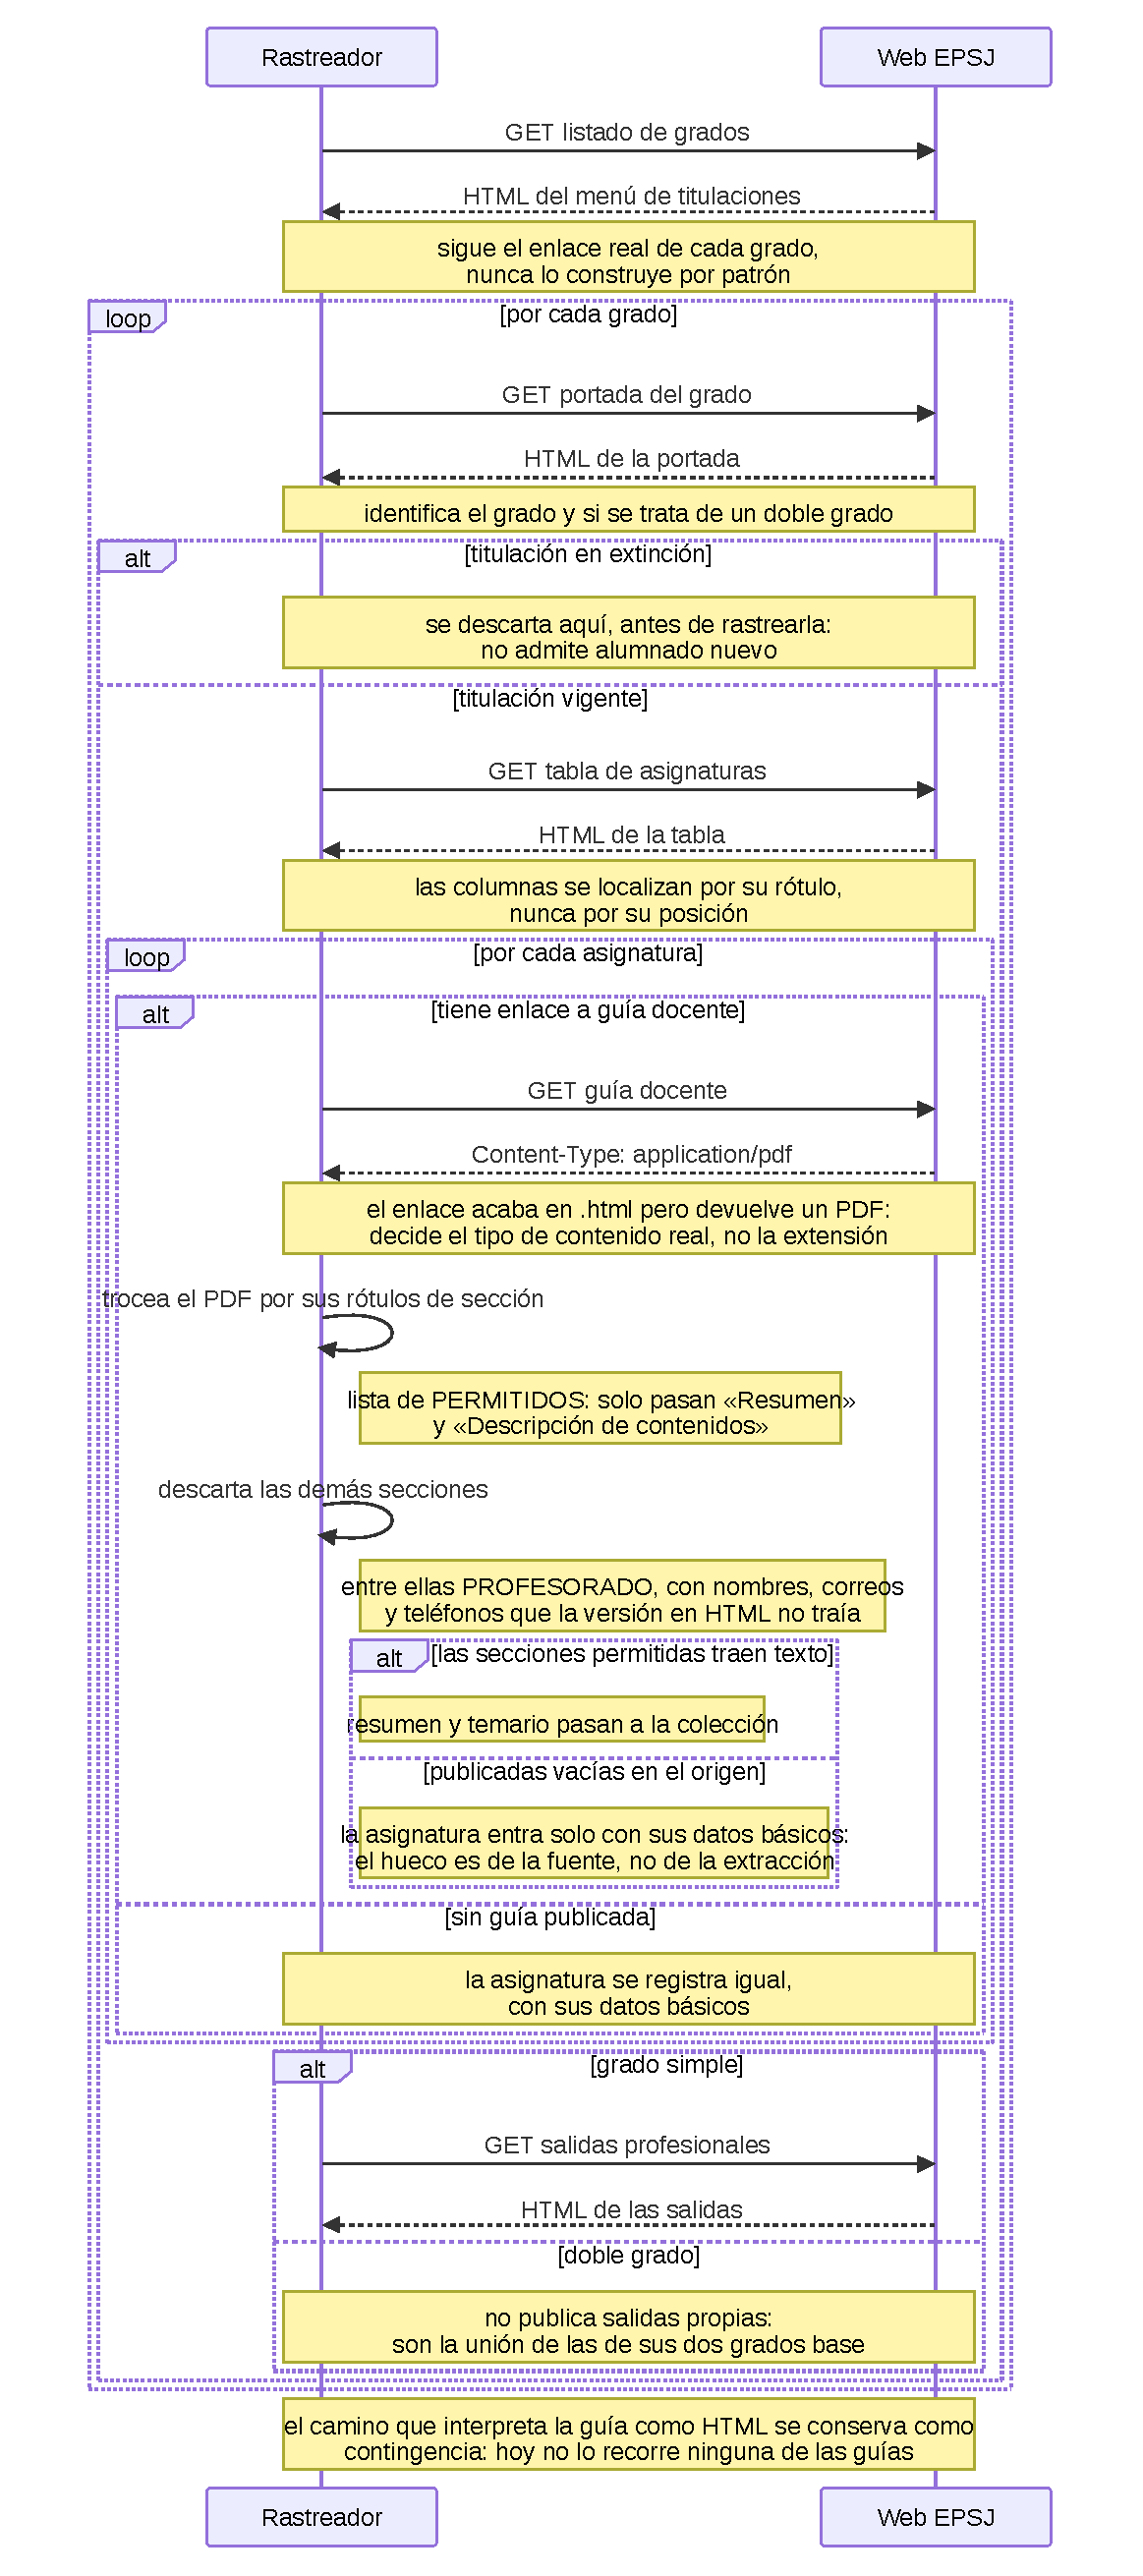
\includegraphics[height=0.9\textheight]{imagenes/Diagrama_secuencia_scraping.pdf}
  \caption[Secuencia del proceso de \textit{scraping} de una guía docente]{Diagrama de secuencia del \textit{scraping}, con sus tres ramas alternativas: asignatura con guía docente frente a sin guía, guía con la estructura esperada frente a un resumen general de la página, y grado simple frente a doble grado. Fuente: Elaboración propia.}
  \label{fig:secuencia_scraping}
\end{figure}

\subsection{Extracción de las guías docentes}

La extracción de las guías docentes es la etapa donde se concentran las anomalías en el contenido aportado por el servidor.
El primer obstáculo es de codificación: cada guía declara en su etiqueta \texttt{<meta>} estar codificada en UTF-8,
pero el servidor de la universidad la sirve realmente en ISO-8859-1. Esto llevaba a múltiples fallos, dado que corrompía las eñes y tildes del idioma español.
Scrapy resuelve el problema sin código adicional porque prioriza la cabecera HTTP \texttt{Content-Type} sobre esa declaración,
tal y como se justificó al elegirlo y se documenta en la sección \ref{sec:eleccion_herramientas}.

El contenido de interés (resumen, requisitos previos y temario) se localiza por el identificador
de su sección dentro del HTML de la guía, y no por su posición en el documento: la posición varía entre titulaciones,
pero el identificador es estable.

No todas las asignaturas disponen de guía publicada: de las 361 asignaturas del catálogo,
296 cuentan con guía docente y 65 no la tienen todavía (una cobertura en torno al 82 \%).
Estas 65 se concentran en las titulaciones de implantación reciente, cuyos cursos superiores aún no
han publicado sus guías, como ocurre en el Grado en Inteligencia Artificial y Ciberseguridad. Además,
en 5 de las 296 guías la estructura esperada no aparece; en esos casos se activa un mecanismo de
respaldo que conserva la información disponible en lugar de descartar la asignatura.

\begin{borrador}
  \item \textbf{Fase:} 1 (IT-95) --- \emph{esta subsección entera describe un
        mecanismo que ya no es el que se usa}. Todo lo de arriba cuenta la
        extracción desde HTML; medido el 29/07/2026 sobre el rastreo del curso
        2026-27, \textbf{las 288 guías del corpus vienen de PDF y ninguna de
        HTML}. Hay que reescribirla contando los dos caminos y cuál está vivo.
  \item La comprobación no es una estimación: el camino HTML une sus bloques con
        doble salto de línea y el limpiador colapsa todo espacio en blanco, así
        que un texto sacado del HTML no puede contener un salto suelto. No hay ni
        un doble salto en todo el corpus y sí 564 campos con saltos simples.
  \item Consecuencia que hay que enunciar: el módulo de extracción de PDF dejó de
        ser un caso particular y es por donde pasa \textbf{el 100 \% del contenido}.
        Sus 17 rótulos de sección, escritos a mano contra una plantilla observada,
        sostienen ahora la colección entera.
  \item El camino HTML no se retira: la fuente ha cambiado de formato dos veces en
        un año y podría volver. Pero pasa a declararse como \emph{contingencia sin
        uso real}, no como parte del flujo. Afecta al umbral de contenido, al
        mecanismo de respaldo y al campo \texttt{cuerpo\_general}, que no se
        activan nunca con el corpus actual (0 respaldos de 288 guías).
  \item Las cifras 361/296/65 y el 82 \% son las del snapshot de julio de 2026,
        curso 2025-26. Hay que sustituirlas por las del rastreo definitivo y decir
        de qué fecha y de qué curso son, no darlas como atemporales.
  \item La frase sobre <<5 guías donde la estructura esperada no aparece>> ya no
        describe lo que pasa: hoy el respaldo no se activa ninguna vez. Lo que sí
        hay son 5 asignaturas cuya guía se publica con las secciones de contenido
        \emph{vacías en el origen} (ver el Capítulo~\ref{cap:resultados}).
\end{borrador}

\begin{borrador}
  \item \textbf{Fase:} 1 (IT-96) --- decisión pequeña pero que vale como ejemplo
        del criterio general del proyecto, así que merece un párrafo aquí.
  \item La Escuela añadió en el curso 2026-27 un segundo enlace dentro de la celda
        del nombre de la asignatura (a un documento <<Syllabus>>). Como el nombre
        se componía juntando todo el texto de la celda, ese rótulo se pegaba al
        final y 43 de las 350 asignaturas quedaron con un nombre que no existe.
  \item El primer arreglo borraba ese rótulo concreto. Se sustituyó por otro que no
        depende de cómo se llame: \textbf{el nombre es el texto del mismo enlace
        del que ya salía la dirección de su guía}. Cualquier otro enlace de la
        celda queda fuera por construcción.
  \item Es el mismo criterio que se adoptó para las guías en PDF: no una lista de
        lo que hay que excluir, sino tomar únicamente lo que se sabe que es válido.
        Conviene enunciarlo una vez como principio y referirlo desde los dos sitios.
\end{borrador}

\subsection{Extracción de las salidas profesionales}

Las salidas profesionales se extraen como un bloque de texto por titulación. El catálogo produce 8 bloques de salidas,
uno por cada grado simple con contenido propio. Los dobles grados son un caso particular: no publican salidas profesionales propias,
sino que su perfil de egreso es la unión de las salidas de los dos grados simples que los componen.
Se comprobó contra los datos reales que esa unión es exacta, de modo que las salidas de un doble grado se reconstruyen a
partir de las de sus grados base en lugar de almacenarse por duplicado.

\subsection{Troceado y deduplicación de la colección}
\label{subsec:chunking}

Los modelos de incrustaciones operan sobre una \gl{ventana de contexto} limitada, por lo que la colección
no puede indexarse documento a documento tal y como se recoge desde la página web: es necesario dividir cada texto en fragmentos (\textit{chunks}).
El tamaño del fragmento es un compromiso: uno demasiado grande diluye la \gl{señal semántica} y satura la ventana de contexto,
mientras que uno demasiado pequeño pierde el contexto necesario para que el fragmento tenga sentido por sí solo.

La decisión no se tomó a ciegas, sino midiendo antes la colección y haciendo uso de la estadística: las 296 guías docentes tienen
una mediana de 2\,677 caracteres de contenido, un percentil 90 de 6\,450 y un máximo de 23\,940. Los modelos de incrustaciones
multilingües habituales admiten en torno a 512 \glr{tokens}{token}, unos 2\,000 caracteres en español, de manera que más de
la mitad de las guías no cabe en un único fragmento. A esa restricción de tamaño se suma una restricción de diseño que el sistema no puede violar:
un fragmento nunca puede mezclar contenido de dos asignaturas distintas, porque un fragmento así recuperado atribuiría a una asignatura el temario de otra.

Con esas dos condiciones sobre la mesa se compararon cuatro estrategias,
recogidas en la Tabla~\ref{tab:alternativas_chunking}. El razonamiento completo, con la evidencia que respalda cada descarte,
se documentó en el registro de decisión de arquitectura ADR-0001\cite{repo_tfg}.

\begin{table}[H]
  \centering
  \small
  \caption{Estrategias de fragmentación consideradas (ADR-0001).}
  \label{tab:alternativas_chunking}
  \begin{tabularx}{\textwidth}{@{}>{\raggedright\arraybackslash}p{3.2cm} X@{}}
    \toprule
    \textbf{Estrategia} & \textbf{Descripción del método} \\
    \midrule
    Tamaño fijo con solape &
    Corta el texto cada $n$ tokens con ventana de solape. Simple, pero rompe frases y puede mezclar dos asignaturas en un mismo fragmento. \\
    \addlinespace
    Estructural por unidad semántica &
    Parte de la unidad docente (guía o bloque de salidas) y solo subdivide si excede el máximo, cortando por fronteras naturales. Respeta los límites entre asignaturas por construcción. \\
    \addlinespace
    Semántica por incrustaciones &
    Detecta cambios de tema comparando \emph{embeddings} de frases consecutivas.\\
    \addlinespace
    Un fragmento por asignatura &
    Sin subdivisión. El 50\,\% de las guías supera los 2\,677 caracteres (máx.\ 23\,940), por lo que la incrustación truncaría contenido en silencio.\\
    \bottomrule
  \end{tabularx}
\end{table}



Ya en la estrategia elegida, el algoritmo parte de la unidad completa y solo la divide cuando hace 
falta: primero corta por párrafos y, si algún fragmento sigue superando el tamaño máximo, lo subdivide por frases; 
por último fusiona con sus vecinos los fragmentos residuales que se han quedado demasiado cortos y reequilibra el par resultante. 
A cada fragmento se le antepone un encabezado autocontenido con el nombre de la asignatura, su tipo, sus créditos ECTS y 
la titulación, de forma que conserve el sentido cuando se recupere aislado del resto. Los parámetros de partida son 1\,200 caracteres de tamaño objetivo,
1\,500 de máximo (contando el encabezado), y 200 de mínimo. El máximo es una restricción dura, mientras que el mínimo es solo una preferencia,
ya que una unidad más corta que ese umbral no se puede alargar.

\textcolor{borrador2}{Esa jerarquía deja de ser una declaración de intenciones en el caso en que
las dos condiciones no se pueden satisfacer a la vez. Cuando dos fragmentos consecutivos no caben
juntos bajo el máximo y el texto tampoco ofrece una frontera por la que repartirlos de otra manera,
el procedimiento conserva el fragmento corto en lugar de forzar la unión: incumplir una preferencia
de calidad es admisible, mientras que superar el máximo haría que el modelo de incrustaciones
truncase el fragmento en silencio y se perdiera contenido sin que nada lo advirtiera. Reconocer ese
caso es además lo que garantiza que el procedimiento termine, ya que solo vuelve a empezar cuando
el número de fragmentos ha disminuido de verdad.}

\begin{borrador}                                
  \item \textbf{Fase:} 1 (IT-28/IT-29). Cuando se elija el modelo de embeddings hay que revisar y seguramente cambiar el tamaño máximo contra su ventana de contexto real y contrastar objetivo/mínimo con las métricas de recuperación del experimento comparativo.
\end{borrador}

La Figura~\ref{fig:secuencia_chunking} recoge este proceso completo sobre el conjunto de datos ya extraído. Antes de trocear nada, se agrupan las guías por su nombre y su contenido, para deduplicar las que se comparten entre titulaciones, según se explica más adelante. Después, por cada grupo de guía, se decide el encabezado del fragmento: si se encuentran los datos de la asignatura, el encabezado incluye su nombre, tipo, créditos ECTS y titulaciones, y si no se encuentran, se usa un encabezado más genérico con solo el nombre. El texto completo de la guía se divide y se empaqueta hasta el tamaño objetivo, y los fragmentos que quedan por debajo del mínimo se fusionan con su vecino y se reequilibran. Cada unidad devuelve así sus fragmentos numerados.

El diagrama recoge además las dos ramas que no siguen ese camino principal. Las salidas profesionales de cada grado se trocean igual que una guía, pero con un encabezado propio. Las asignaturas sin guía docente no se descartan en silencio: cada una genera un único fragmento informativo que recoge sus datos básicos, de modo que el sistema pueda al menos nombrarla y situarla en su titulación en lugar de comportarse como si no existiera.


\begin{figure}[H]
  \centering
  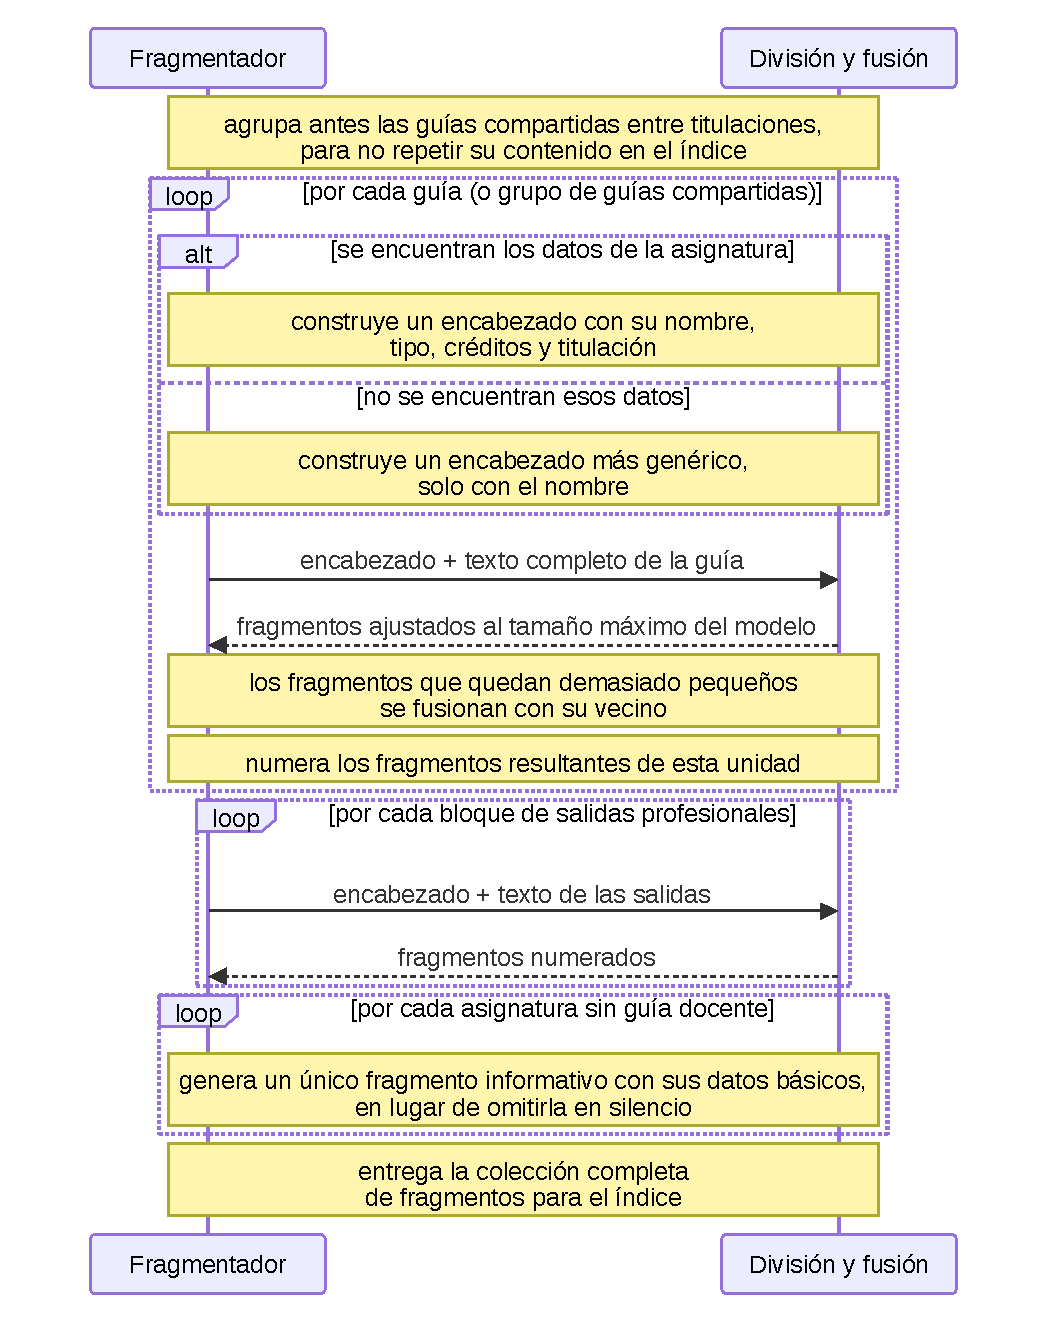
\includegraphics[width=\textwidth]{imagenes/Diagrama_secuencia_chunking.pdf}
  \caption[Secuencia del proceso de troceado y deduplicación]{Diagrama de secuencia del troceado y la deduplicación de la colección, con las ramas de salidas profesionales y de asignaturas sin guía docente. Fuente: Elaboración propia.}
  \label{fig:secuencia_chunking}
\end{figure}

La Figura~\ref{fig:estructura_chunk} desglosa esa estructura sobre un fragmento real de la colección. La distinción
importante es la de la izquierda frente a la derecha: solo el campo \texttt{texto} (encabezado más cuerpo) se convierte en
vector, mientras que el resto de campos acompañan al fragmento sin intervenir en la búsqueda, y sirven para saber de dónde
salió cada respuesta.


\begin{figure}[H]
  \centering
  \resizebox{\textwidth}{!}{%
  \begin{tikzpicture}[                                                                                                                      
      font=\footnotesize,
      bloque/.style={draw=diagNodoBorde, fill=diagNodo, align=left,
          inner sep=7pt, rounded corners=2pt},
      titulo/.style={font=\footnotesize\bfseries, anchor=north west,
          text=diagGrupoBorde!55!black}
    ]
    % --- Columna izquierda: el campo que se incrusta ---
    \node[bloque, text width=9.2cm] (enc) {%
      \textbf{Encabezado autocontenido} \hfill \textit{generado, no extraído}\\[3pt]
      <<Automática industrial>>, asignatura obligatoria de 6 ECTS impartida en
      4 titulaciones: Grado en Ingeniería Electrónica Industrial; Grado en
      Ingeniería Eléctrica; Grado en Ingeniería Mecánica; Grado en Ingeniería
      de Organización Industrial.};
    \node[bloque, text width=9.2cm, below=4mm of enc.south west,
      anchor=north west] (cue) {%
      \textbf{Cuerpo} \hfill \textit{texto de la guía docente}\\[3pt]
      Conceptos básicos 2.1 Sistemas de eventos discretos 2.2 Concepto de
      estado y transición 2.3 Álgebra de Boole 2.4 Automatismos 2.5
      Automatismos combinacionales\dots};
    
    % --- Columna derecha: metadatos ---
    \node[bloque, text width=5.6cm, right=9mm of enc.north east,
    anchor=north west] (met) {%
    \textbf{Metadatos}\\[3pt]
    \texttt{origen}: guia\\
    \texttt{nombre}: Automática industrial\\
    \texttt{grados}: [4 titulaciones]\\
    \texttt{codigos}: [13112002, 13512002,\\ \hphantom{\texttt{codigos}: [}13412001, 13012001]\\
    \texttt{chunk\_index}: 1\\
    \texttt{total\_chunks}: 4};
    
    % --- Agrupaciones ---
    \begin{scope}[on background layer]
      \node[grupoDiag, rounded corners=3pt, fit=(enc)(cue)] (gtxt) {};
      \node[grupoDiag, rounded corners=3pt, fit=(met)] (gmet) {};
    \end{scope}
    \node[titulo, anchor=south west] (ltxt)
    at ([yshift=1.4mm]gtxt.north west) {campo \texttt{texto}: lo único que se convierte en vector};
    \node[titulo, anchor=south west] (lmet)
    at ([yshift=1.4mm]gmet.north west) {acompañan al vector, no se buscan};
    
    % --- Marco exterior (engloba también los rótulos de cada grupo) ---
    \begin{scope}[on background layer]
      \node[draw=diagNodoBorde, thick, rounded corners=4pt, inner sep=9pt,
        fit=(gtxt)(gmet)(ltxt)(lmet)] (marco) {};
    \end{scope}
    \node[font=\footnotesize\bfseries, anchor=south west]
    at ([yshift=1.8mm]marco.north west)
    {Fragmento 1 de 4 de <<Automática industrial>> --- máximo 1\,500 caracteres, encabezado incluido};
  \end{tikzpicture}%
  }
  \caption[Estructura de un fragmento (\textit{chunk})]{Estructura de un
    fragmento de la colección, sobre un caso real de \texttt{chunks.json}. El
    encabezado se antepone al cuerpo para que el fragmento siga teniendo sentido
    al recuperarse aislado; los campos \texttt{grados} y \texttt{codigos} son
    listas porque esta guía está deduplicada y se imparte en cuatro
    titulaciones. Fuente: Elaboración propia.}
  \label{fig:estructura_chunk}
\end{figure}

Al revisar los datos extraídos apareció un problema que hacía ineficiente el corpus: buena parte de las guías son contenido repetido,
porque asignaturas de primeros cursos como Matemáticas I o Física se imparten en varias titulaciones con la misma guía carácter por carácter, esto pasa puesto que muchas titulaciones de primero y segundo de ingeniería tienen las mismas asignaturas.
En concreto, 96 de las 296 guías se agrupan en 28 conjuntos que comparten nombre y contenido, de modo que 68 de ellas son copias de otra.
La redundancia tiene un efecto directo sobre la recuperación: hasta cuatro copias idénticas podrían ocupar los primeros puestos del \textit{ranking} y
expulsar resultados diversos. La respuesta fue deduplicar dentro del fragmentador, dejando una sola unidad por conjunto que arrastra la lista de
titulaciones en las que se imparte; de ahí que los campos \texttt{grados} y \texttt{codigos} de un fragmento sean listas y no cadenas.

Deduplicar exige decidir cuándo dos guías se consideran la misma. Se plantearon dos claves de agrupación, comparadas
en la Tabla~\ref{tab:claves_dedup}: agrupar únicamente por el contenido del texto, o exigir además que coincida el nombre de la
asignatura. La elegida es la segunda, el par (nombre, contenido), y el motivo es un caso real: el mecanismo de respaldo descrito
más arriba puede generar un texto idéntico para dos asignaturas que no tienen nada que ver. Es lo que ocurre entre
\textit{Smart Grids. Redes Eléctricas Inteligentes} y \textit{Técnicas de ingeniería gráfica aplicadas a ingeniería eléctrica},
ambas del Grado en Ingeniería Eléctrica, que comparten el cuerpo de guía docente sin ser en absoluto la misma
materia. Agrupar solo por contenido las habría fusionado en una única unidad, con lo que una consulta sobre redes eléctricas
inteligentes podría devolver el temario de dibujo técnico.

% !TEX root = ../main.tex
\begin{table}[htbp]
  \centering
  \small
  \caption{Claves de deduplicación consideradas (ADR-0001).}
  % Cifras medidas sobre data/grados.json, rastreo del 05/08/2026, curso 2026-27.
  % Conjuntos: grupos con mas de una guia. Copias: guias que la deduplicacion retira
  % (288 - unidades resultantes). Con la clave elegida quedan 210 unidades; con la
  % descartada, 207.
  \label{tab:claves_dedup}
  \begin{tabularx}{\textwidth}{@{}>{\raggedright\arraybackslash}p{3.1cm} c c Y@{}}
    \toprule
    \textbf{Clave}      & \textbf{Conjuntos} & \textbf{Copias} & \textbf{Comportamiento observado}                      \\
    \midrule
    Solo contenido      & 41                 & 81              & 
    Agrupa las tres parejas dudosas, incluida la que no debe agruparse. Descartada.                                     \\
    \addlinespace
    (nombre, contenido) & 38                 & 78              & 
    Evita la fusión errónea a costa de dejar sin agrupar dos parejas que sí eran la misma asignatura. \textbf{Elegida}. \\
    \bottomrule
  \end{tabularx}
\end{table}


Esos tres conjuntos de diferencia entre una clave y otra (31 frente a 28) son exactamente las tres parejas que tienen el
mismo contenido pero distinto nombre, y conviene mirarlas una a una porque no todas son del mismo tipo. Dos son errores de la
clave elegida, y son dos parejas independientes entre sí, no relacionadas: <<Fundamentos de la programación>> frente a
<<Fundamentos de programación>>, y <<Fundamentos físicos de la Informática>> frente a <<Fundamentos físicos de la informática>> (solo cambia la inicial de <<informática>>). En ambos casos se trata de la misma asignatura escrita de dos maneras, y exigir que el nombre coincida impide
agruparlas. La tercera es la pareja del Grado en Ingeniería Eléctrica
citada antes, donde no agrupar es lo correcto. El balance, por tanto, es de dos falsos negativos a cambio de evitar un falso
positivo, y se acepta a propósito porque los dos errores no cuestan lo mismo: fusionar dos asignaturas distintas corrompe el
índice y puede hacer que el sistema atribuya un temario a quien no le corresponde, mientras que no fusionar dos copias
idénticas solo deja el índice ligeramente más grande.

El efecto sobre la colección, medido sobre el conjunto de datos completo, es una reducción de 1\,172 a 892 fragmentos,
un 24 \% menos. De esos 892, 818 proceden de guías docentes, 65 son fragmentos informativos de las asignaturas que todavía no
tienen guía publicada y 9 corresponden a salidas profesionales. Los 280 fragmentos eliminados suponen el 25 \% de los 1\,098 que
las guías generaban antes de deduplicar. Los tamaños resultantes van de 227 a 1\,499 caracteres, con una mediana de 1\,093 y
ningún fragmento por encima del máximo.

\textcolor{borrador2}{Decidir cuándo dos guías son la misma no es lo único que obliga a fijar un
criterio de identidad. El fragmentador necesita además localizar, para cada guía, la asignatura de
la que salen los metadatos del encabezado, y esa búsqueda se hacía por el par (titulación, código).
El código, sin embargo, no siempre está publicado: 57 asignaturas de los planes de implantación
reciente no lo tienen, y todas ellas caían bajo la misma clave dentro de su titulación, de modo que
la última sobrescribía a las anteriores sin que nada avisara. En el plan de 2025 del Grado en
Ingeniería Geomática y Topográfica eran 18 asignaturas reducidas a una sola entrada, y 38 en el
Grado en Inteligencia Artificial y Ciberseguridad. Si alguna de ellas llegara a publicar su guía, el
encabezado resultante atribuiría el temario a una materia distinta, y lo haría dentro del campo
\texttt{texto}, que es justamente el único que se convierte en vector. La clave pasó a ser el par
(titulación, código o nombre) --- la misma que ya usaban el rastreador y el verificador de
fragmentos --- y se recogió en una única función para que los tres módulos identifiquen una
asignatura de la misma manera.}

\section{Verificación y reproducibilidad de la Fase 0}
\label{secc:verificacion_fase0}

\begin{borrador}                                                                                                                  
  \item \textbf{Fase:} 0 (IT-19) --- redactado. Recordatorio al revisar: aquí \textbf{no} van cifras de caracterización de la colección ni amenazas a la validez; eso es IT-58 y va al Capítulo~\ref{cap:resultados} en la Fase 2.
\end{borrador}

La fiabilidad de la Fase 0 recae en dos verificadores que se ejecutan sobre el conjunto de datos completo. El primero, \texttt{check\_dataset.py}, comprueba la integridad de grados, asignaturas, guías y salidas: el número de entidades, la presencia de los campos obligatorios y la validez de los tipos de asignatura. El segundo, \texttt{check\_chunks.py}, verifica los tamaños de los fragmentos y la corrección de la deduplicación. Ambos se ejecutan en local antes de cada subida al repositorio, mientras que la integración continua en la nube ejecuta la batería de pruebas unitarias (\texttt{pytest}) y la comprobación de tipos (\texttt{mypy}).

Las pruebas unitarias se emplean en base a los ficheros reales descargados llamados \textit{fixtures} de la web de la EPSJ. Es una decisión deliberada: los datos sintéticos no reproducen las anomalías reales de la fuente. Cada defecto encontrado se incorpora como caso de regresión con su HTML real.

\textcolor{borrador2}{Los verificadores, sin embargo, solo protegen de aquello que efectivamente miran.
Al revisar el criterio de identidad del fragmentador se comprobó que \texttt{check\_chunks.py}
respondía que el corpus era correcto aun teniendo los encabezados cruzados: lo que comparaba eran
las claves que relacionan cada fragmento con su asignatura, y esas sí cuadraban, mientras que el
error estaba en el texto del encabezado, que no revisaba nadie. La comprobación que faltaba --- que
cada fragmento empiece por el nombre de su propia unidad --- se añadió junto con la corrección. El
patrón es el mismo que el de los defectos descritos más arriba, y conviene enunciarlo así de claro:
un verificador puede estar midiendo algo distinto de lo que se cree que mide, y mientras tanto
devuelve un resultado correcto.}

\textcolor{borrador2}{Para poder afirmar algo sobre el conjunto de datos hace falta saber de cuándo
es. Hasta IT-90 no había ninguna fecha dentro de los ficheros: la única constancia era una nota
escrita a mano y no versionada, de modo que copiar el conjunto de datos a otro sitio hacía perder
su procedencia y olvidar actualizar la nota la falseaba. El rastreador registra ahora la fecha de
extracción, y cada guía docente lleva el curso académico al que pertenece. Ese curso no se escribe
a mano en ninguna parte: se deduce de la propia dirección de la ficha en el catálogo de la
Universidad, que lo incluye en su ruta, con lo que un dato tomado de la fuente no puede quedarse
obsoleto sin que nadie lo advierta. Cuando la dirección no lo indica, el campo queda vacío en lugar
de suponer un curso, con el mismo criterio que se aplica al crédito ausente. Los cursos presentes
se enumeran todos y no se resumen a uno solo, porque la Escuela publica las guías del curso nuevo a
medida que las tiene y un mismo rastreo puede recoger dos, algo que conviene declarar antes que
dejar implícito.}

La reproducibilidad del sistema no se apoya en una copia versionada de los datos (no está subida a github), sino en el propio pipeline: el conjunto de datos no se versiona y se regenera bajo demanda ejecutando el rastreador y, a continuación, el fragmentador. La separación entre rastreador (\textit{spider}) y fragmentador (\textit{chunker}) es intencionada: volver a fragmentar es barato y se repite muchas veces durante la experimentación, mientras que volver a rastrear la web es costoso y poco respetuoso con el servidor de la universidad. Por eso ambos son módulos independientes, como se argumenta en el ADR-0001.

\begin{borrador}
  \item \textbf{Fase:} 2 (IT-58) --- matiz honesto sobre esta afirmación, para
        adelantarse al tribunal. El 24/07/2026 se comprobó que re-rastrear la web
        \emph{no} reproduce el mismo corpus: la fuente había cambiado dos veces
        (guías del curso 2026-27 servidas en PDF, resuelto en IT-67; y dos
        titulaciones de Geomática con la tabla de asignaturas reestructurada,
        resuelto en IT-76 e IT-77). Es decir, el pipeline reproduce <<el estado
        actual de la fuente>>, que no es lo mismo que <<el corpus sobre el que se
        hicieron los experimentos>>: eso es una limitación de la reproducibilidad
        que conviene enunciar, no un defecto que se pueda corregir.
  \item Lo que sí se ha corregido es la mitad que dependía del proyecto: desde
        IT-90 el propio conjunto de datos lleva dentro su fecha de extracción y
        su curso, así que ya no hace falta acordarse de decirlo por fuera. Queda
        pendiente para IT-58 dar esa fecha y ese curso al caracterizar el corpus,
        en vez de presentarlo como atemporal.
\end{borrador}